\documentclass[a4paper,10pt,italian]{article}
\textwidth 460pt
\textheight 700pt
\hoffset -60pt
\voffset -80pt

\usepackage[italian]{babel}
\usepackage{graphicx}
\usepackage{textcomp}
\usepackage{amsmath}
\usepackage{amssymb}
\usepackage{epstopdf}

%\usepackage{fancyhdr} % This should be set AFTER setting up the page geometry
%\pagestyle{fancy} % options: empty , plain , fancy

\newcommand{\D}[0]{\mathfrak D}
\newcommand{\s}[0]{\mathfrak S}
\newcommand{\F}[0]{\mathfrak F}

\title{Analisi D for Dummies}
\author{bug report: \emph{mario.piccinelli@gmail.com}}
\begin{document}

\maketitle

\thanks{
Quest'opera � stata rilasciata sotto la licenza Creative Commons Attribuzione 2.5 Italia. Per leggere una copia della licenza visita il sito web http://creativecommons.org/licenses/publicdomain/ o spedisci una lettera a Creative Commons, 559 Nathan Abbott Way, Stanford, California 94305, USA.
}

\tableofcontents

\newpage

%---------------------------------------------------------------------------------------------

\section{Funzioni di una variabile complessa}
\begin{align*}
    f:\quad&\Omega\rightarrow C &\Omega\subset C  \\
    &z\in\Omega\rightarrow f(z)\in C  
\end{align*}
$z\in C \Rightarrow z=x+iy$\quad $x,y\in R$\\
$x=\Re(z)\quad y=\Im(z)$

\begin{figure}[htbp] 
   \centering
   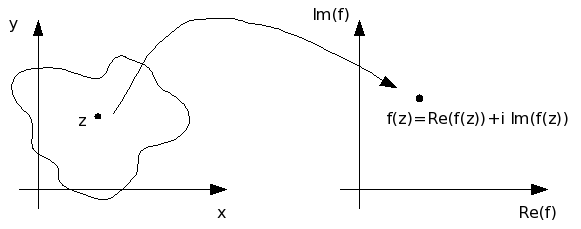
\includegraphics[height=3cm]{funzioneUnaVariabile.png} 
 \end{figure}
 
\noindent\textbf{Modulo} di z: $\mid z\mid =\sqrt{x^2+y^2}\geq 0$\\\\

\subsection{Definizioni}

\subsubsection{Distanza}
\textbf{Distanza} tra $z_1$ e $z_2$: 
$$ dist(z_1,z_2)=\mid z_1-z_2\mid=\sqrt{(x_1-x_2)^2+(y_1-y_2)^2}=\sqrt{\mid x_1-x_2\mid^2+\mid y_1-y_2\mid^2} $$

\subsubsection{Palla aperta}
\textbf{Palla aperta} di centro $z_0$ e raggio $R$:
$$B_R(z_0)=\{z\in C\quad:\quad\mid z-z_0\mid< R\}$$
\begin{figure}[htbp] 
   \centering
   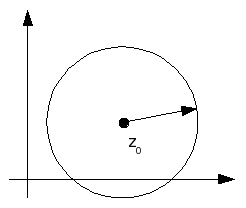
\includegraphics[height=4cm]{palla.png} 
 \end{figure}
 
\subsubsection{Palla chiusa}
\textbf{Palla chiusa} di centro $z_0$ e raggio $R$:
$$\overline{B_R(z_0)}=\{z\in C\quad:\quad\mid z-z_0\mid< R\}$$

\subsubsection{Circonferenza}
\textbf{Circonferenza} di centro $z_0$ e raggio $R$:
$$C_R(z_0)=\overline{B_R(z_0)}- B_R(z_0)\quad=\quad\{z\in C \quad:\quad\mid z-z_0\mid=R\}$$

\subsubsection{Punto interno}
Definizione: $z_0\in\Omega\subset C$ \'e un \underline{punto interno} di $\Omega$ se:
$$\exists R>0 \quad:\quad B_R(z_0)\subset C$$

\paragraph{Esempio}
$\Omega=B_1(1)\cup B_1(-1)\cup \{0\}$

\begin{figure}[h] 
   \centering
   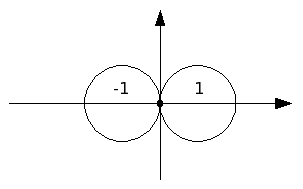
\includegraphics[height=4cm]{palla2.png} 
 \end{figure}

\noindent$z_0=0$ NON \'e un punto interno di $\Omega$ (non esiste una palla centrata in $z_0$ che sia interna a $\Omega$)\\
$z'_0=1+i\frac{1}{2}$ \'e un punto interno

\paragraph{Esempio}
$\Omega=B_R(z_0)$

\begin{figure}[h] 
   \centering
   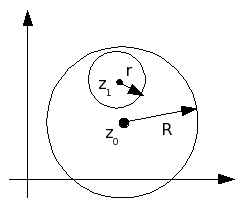
\includegraphics[height=4cm]{palla1.png} 
\end{figure}

\noindent Si vede che \emph{qualunque} punto $z_1$ della palla aperta \'e un punto interno, poich\'e:
$$B_R(z_1)\subset B_R(z_0) \quad \mbox{per ogni } r<R-\mid z_0-z_1\mid$$
\\\\
\subsubsection{Insieme aperto}
$\Omega\subset C$ \'e un \underline{insieme aperto} se ogni suo punto \'e un punto interno.

\newpage

\subsubsection{Punto di accumulazione}
Dato $\Omega\subset C$ un punto $z_0\in C$ \'e un \underline{punto di accumulazione} per $\Omega$ se 
$$\forall R>0\quad B_R(z_0) \mbox{ contiene punti di }\Omega$$
eventualmente diversi da $z_0$.

\paragraph{Esempio:}
$\Omega_2=B_1(1) \cup B_1(-1)$
   
\begin{figure}[h] 
   \centering
   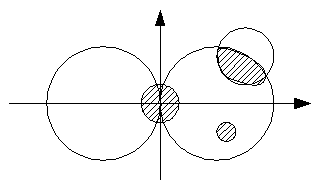
\includegraphics[height=4cm]{palla3.png} 
\end{figure}

I punti indicati sono tutti punti di accumulazione.\\\\
NB: $z_0$ punto interno di $\Omega$ implica $z_0$ punto di accumulazione\\
Questo implica che un insieme aperto \'e formato solo da punti interni.\\\\
inoltre se $\Omega$ ha un punto di accumulazione, allora $\Omega$ ha infiniti punti.
\\\\
\subsection{Limite}
$f:\Omega\in C \rightarrow C\quad z_0\in C$ punto di accumulazione per $\Omega$

\begin{figure}[h] 
   \centering
   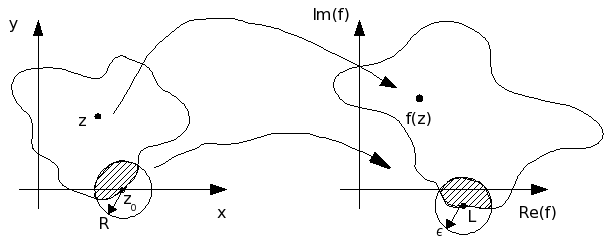
\includegraphics[height=5cm]{limite.png} 
\end{figure}

\noindent$f$ ha un limite finito per $z$ tendente a $z_0$
$$\lim_{z\to z_0} f(z)=L\quad \in C$$
se
$$\forall \varepsilon>0 \quad \exists R>0\quad:\quad \mid f(z)-L\mid<\varepsilon\quad \forall z\in \Omega\cap B_R(z_0)\quad z\neq z_0 $$
\\\\
\subsection{Continuit\'a}
$f:\Omega\rightarrow C\quad \Omega\subset C \mbox{ aperto}\quad z_0\in \Omega$\\\\
$f$ \'e \underline{continua} in $z_0$ se $\lim_{z\to z_0}f(z)=f(z_0)$
$$\forall \varepsilon>0 \quad\exists R>0 \quad:\quad \mid f(z)-f(z_0)\mid<\varepsilon\quad\forall z\in\Omega\hat B_R(z_0)$$
\\\\
\subsection{Derivabilit\'a}
$f:\Omega\rightarrow C\quad \Omega\subset C \mbox{ aperto}\quad z_0\in \Omega$\\\\
$f$ \'e \underline{derivabile} in $z_0$ se $\exists$ finito 
$$ \frac{f(z)-f(z_0)}{z-z_0}=f'(z_0) $$

\paragraph{Esempio}
$f(z)=z^2\quad f:C\rightarrow C\quad$ derivabile in tutto $C$\\\\
Scrivendo $z=z_0+h$ (con $h\in C$) ho 
$$f'(z_0) = \lim_{h\to0}\frac{f(z_0+h)-f(z_0)}{f} = \lim_{h\to0}\frac{(z_0+h)^2-z_0^2}{h} = \lim_{h\to0}\frac{z_0^2+2z_0h+h^2-z_0^2}{h}=\lim_{h\to0}(2z_0+h)=2z_0$$

\paragraph{Esempio}
$f(z)=\Re(z) \quad f:C\to C$\\\\
$z=x+iy\quad\to\quad f(z)=x$
$$f'(z)=\lim_{h\to0}\frac{f(z_0+h)-f(z_0)}{h}=\lim_{h\to0}\frac{\Re(z_0+h)-\Re(z_0)}{h}=\lim_{h\to0}\frac{\Re(h)}{h}$$
\begin{itemize}
  \item h puramente reale $\lim_{h\to0}\frac{\Re(h)}{h}=1$
  \item h puramente immaginaria $\lim_{h\to0}\frac{0}{h}=0$
\end{itemize}
Poich\'e il limite non \'e definito (ho due risultati diversi) la funzione non \'e derivabile $\forall z_0$

\newpage

\subsection{Differenziabilit\'a}
f \'e \underline{differenziabile} in $z_0$ se:
$$\exists \lambda\in C\quad:\quad f(z)=f(z_0)+\lambda\cdot(z-z_0)+R(z-z_0)$$
dove il resto $R(z-z_0)$ soddisfa la seguente:
$$\lim_{z\to z_0}\frac{R(z-z_0)}{z-z_0}=0$$

\begin{figure}[h] 
   \centering
   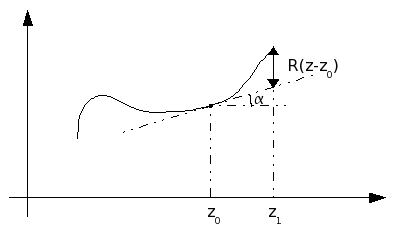
\includegraphics[height=4cm]{differenziale.png} 
\end{figure}

Se $f$ \'e differenziabile in $z_0$, allora $\lambda=\frac{f'}{z_0}$\\\\
$f$ differenziabile implica $f$ derivabile\\\\
Si pu\'o riscrivere cos\'i la definizione:
$$\exists \lambda\in C \quad:\quad f(z_0+h)=f(z_0)+\lambda\cdot h + R(h)$$
Quindi
$$\lim_{h\to0}\frac{R(h)}h=0\quad=\lim_{h\to0}\frac{f(z_0+h)-f(z_0)-\lambda\cdot h}{h}=\lim_{h\to 0}\Bigr(\frac{f(z_0+h)-f(z_0)}{h}-\lambda\Bigr) = 0$$
($R(h)$ \'e detto \underline{o piccolo} di $h$, ovvero $o(h)$ per $h\to0$)\\\\
Il che implica che:
$$\lim_{h\to0}\frac{f(z_0+h)-f(z_0)}h=\lambda$$

\subsection{Teorema di Cauchy-Riemann}
Scrivendo $z=x+iy$, si pu\'o scrivere:
\begin{align*}
	f(z)&=\underbrace{\Re(f(z))}_{u}+i\underbrace{\Im(f(z))}_{v}\\
		&=u(x,y)+iv(x,y)
\end{align*}
In tal modo, la funzione $f$ risulta divisa in due funzioni separate:
\begin{align*}
	f&:C\to C\\
	u&:R^2\to R\\
	v&:R^2\to R
\end{align*}
Quindi, supponendo $f:C\to C$ con $\Omega\subset C$ aperto\\\\
$f$ \'e derivabile in $z$ se e solo se $u$ e $v$ sono differenzibili (come campi scalari) in ($x,y$), e valgono le equazioni:
$$\frac{\delta u}{\delta x}=\frac{\delta v}{\delta y} \quad\quad \frac{\delta u}{\delta y}=-\frac{\delta v}{\delta x}$$
\begin{center}
	\emph{equazioni di Cauchy-Riemann}
\end{center}

\paragraph{Esempio}
$$f(z)=\Re(z)=x\quad [z=x+iy]$$
$$u(x,y)=x$$
$$v(x,y)=0$$
$$\frac{\delta u}{\delta x}=1\not= \frac{\delta v}{\delta y}=0\quad\Rightarrow\quad f\mbox{ non derivabile}$$

\paragraph{Esempio}
$$f(z)=\mid z\mid^2\quad=\quad\mid x+iy\mid^2\quad=\quad x^2+y^2$$
$$u(x,y)=x^2+y^2$$
$$v(x,y)=0$$
$$\frac{\delta u}{\delta x}=2x=\frac{\delta v}{\delta y}=0\quad\Leftrightarrow\quad x=0$$
$$\frac{\delta u}{\delta y}=2y=\frac{\delta v}{\delta x}=0\quad\Leftrightarrow\quad y=0$$
\begin{center}
	$\Rightarrow$ la funzione \'e derivabile solo nell'origine $(0,0)$ 
\end{center}

\paragraph{Esempio}
$$f(z)=e^z=\sum_{n=0}^{\infty}\frac{z^n}{n!}\quad \mbox{oppure}\quad e^{x+iy}=e^xe^{iy}=e^x\cdot(\cos x + i\sin y)$$
$$u(x,y)=e^x\cos y$$
$$v(x,y)=e^x\sin y$$
$$\frac{\delta u}{\delta x}=e^x\cos y=\frac{\delta v}{\delta y}$$
$$\frac{\delta u}{\delta y}=-e^x\sin x=-\frac{\delta v}{\delta x}$$
\begin{center}
	$\Rightarrow f(z)=e^z$ \'e derivabile in tutto $C$
\end{center}

\subsubsection{Dimostrazione}
ipotesi: $f$ derivabile in $z$ $\Leftrightarrow$ differenziabile in $z$
$$\Rightarrow f(z+h)=f(z)+f'(z)\cdot h +o(h)\quad \mbox{per }h\to0\quad\Bigr( \lim_{h\to0}\frac{o(h)}{h}=0 \Bigr)$$ 
\begin{center}
\framebox{
	$u_0=u(x,y)\quad v_0=(x,y)$
}\\
\framebox{
	$u=u(x+h_1,y+h_2)\quad v=v(x+h_1,y+h_2)$
}\\
\framebox{
	$h=(h_1,h_2)\quad o(h)=o(h)+i\cdot o(h)\quad \mbox{ per le propriet\'a di o piccolo}$
}
\end{center}
$$f(z+h)=u+iv=u_0+iv_0+(\alpha+i\beta)(h_1+h_2)+o(h)+io(h)$$
\begin{align*}
	\Rightarrow \quad &u=u_0+\alpha h_1-\beta h_2+o(h) \quad\Rightarrow\quad\mbox{u differenziabile in }(x,y)\\
	&\mbox{e inoltre si vede che }\frac{\delta u}{\delta x}=\alpha\quad \frac{\delta u}{\delta y}=-\beta\\
	\Rightarrow\quad &v+v_0+\beta h_1+\alpha h_2+o(h)\quad \Rightarrow\quad\mbox{v differenziabile in }(x,y)\\
	&\mbox{e inoltre }\frac{\delta v}{\delta x}=\beta\quad\frac{\delta v}{\delta y}=\alpha
\end{align*}
Quindi \'e dimostrato che:
$$\alpha=\frac{\delta u}{\delta x}=\frac{\delta v}{\delta y}$$
$$\beta=\frac{\delta v}{\delta x}=-\frac{\delta u}{\delta y}$$

\subsection{Curve e Cammini in $C$}
Al variare di $t$, il punto $z$ si sposta lungo un percorso $R\in[a,b]$
$$t\to r(r)=\Re(r(t))+\Im(r(t))$$

\begin{figure}[htbp] 
   \centering
   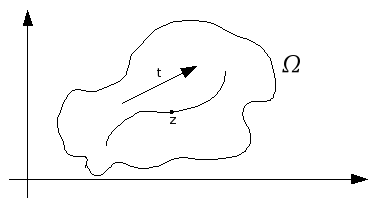
\includegraphics[height=4cm]{curve.png} 
\end{figure}

\subsubsection{$C^1$ a tratti}
$r:[a,b]\to C$ \'e $\mathbf{C^1}$ \textbf{a tratti} se: 
\begin{itemize}
  \item $r$ \'e continua su $[a,b]$
  \item $\exists$ un numero finito di punti $t_1,t_2,\dots,t_n \in ]a,b[$ tali che $t_0=a$ e $t_n=b$ e\\
  	$r(t)$ \'e $C^1$ in $[t_i,t_{i+1}]\quad i=0,1,\dots,n-1$
\end{itemize}

\subsubsection{Curva}
Se $r:[a,b]\to C$ \'e $C^1$ a tratti, allora individua una \textbf{curva} in $C$.\\

\subsubsection{Curve equivalenti}
$r_1:[a_1,b_1]\to C$\\$r_2:[a_2,b_2]\to C$\\\\
$\exists \varphi:[a_2,b_2]\to[a_1,b_1]\quad$ biiettiva, strettamente crescente, $C^1$ a tratti\\
tale che $r_2(t)=r_1((\varphi(t)))\quad\forall t\in[a,b]$\\\\
allora $r_1$ e $r_2$ sono \textbf{curve equivalenti}.\\\\
Esempio:
\begin{align*}
	v_2(t)&=\cos(t)+i\sin(t)\quad&t\in[0,\pi]\\
	v_1(\tau)&=\cos(\tau)+i\sin(\tau)&\tau\in[0,2\pi]\\
	\varphi(t)&=\frac12t:[0,2\pi]\to[0,\pi]
\end{align*}

\subsubsection{Relazione di Equivalenza}
\begin{align*}
	r_1 \sim r_2&\quad\Rightarrow\quad r_2\sim r_1&\mbox{simmetria} \\
	r_1\sim r_1&&\mbox{riflessione}\\
	r_1\sim r_2&\quad e\quad r_2\sim r_3 \quad\Rightarrow\quad\mbox{$r_1$ e $r_3$ sono equivalenti}
\end{align*}

\subsubsection{Classi di equivalenza}
Insieme di tutte le curve equivalenti.

\subsubsection{Curva Orientata}
La \textbf{curva orientata} \'e una classe di equivalenza di funzioni $C^1$ a tratti equivalenti tra loro.\\
L'orientamento \'e il senso di percorrenza uguale per ogni curva della stessa classe.\\
Ognuna delle funzioni della classe di equivalenza \'e detta \textbf{rappresentazione parametrica della curva}.
$$r:[a,b]\to C$$
\begin{itemize}
  \item $r(a)$ e $r(b)$ sono detti \emph{estremi} della curva C.
  \item $r([a,b])$ \'e detto \emph{sostegno} della curva C. 
  \item $r(a)=r(b)$ indica un \emph{cammino chiuso} o \emph{circuito}.
\end{itemize}

\subsubsection{Somma di cammini}
\begin{align*}
	r:[a,b]&\to C&C\\
	r:[a,c]&\to C&C_1\\
	r:[c,b]&\to C&C_2
\end{align*}
con $a<c<b$, allora:
$$C=C_1+C_2$$

\subsubsection{Cammino inverso}
Dato un cammino C con $r:[a,b]\to C$ il \textbf{cammino inverso} ha lo stesso sostegno percorso in senso opposto.\\
Cammino inverso: -C

\subsection{Integrale di una funzione di variabile complessa}
Data una curva C orientata in $C$, $r:[a,b]\to C$, $C^1$ a tratti, suppongo che il mio sostegno sia il dominio di una funzione
$$f:sost(C)\to C \quad \mbox{continua}$$
$$\int_Cf(z)\,dz\quad:=\quad\int_a^bf(r(t))\cdot r'(t)\,dt$$
$$z\in sost(C)\quad z=r(t)$$
Dato che il prodotto $f(r(t))\cdot r'(t)$ risulta continuo a tratti posso esprimere l'integrale come somma di integrali di funzioni continue in ogni intervallo.
$$\sum_{i=0}^{n-1}\int_{t_i}^{t_{i+1}}\underbrace{f(r(t))\cdot r'(t)} _{C_0}\,dt$$
Propriet\'a:
\begin{itemize}
  \item Linearit\'a: $$\int_C(\lambda\cdot f + \mu g)\,dz=\lambda\cdot\int_Cf\,dz+\mu\int_C g\,dz$$
  \item Additivit\'a: $$\int_{C_1+C_2}f(z)\,dz=\int_{C_1}\dots+\int_{C_2}\dots$$
  \item $$\int_{-C}=-\int_{C}$$
\end{itemize}

\subsubsection{Lunghezza di C}
$$l(C)=\int_a^b\mid r'(t)\mid\,dt$$
Fare molta attenzione se la curva presenta parte reale e parte immaginaria!\\\\
Esempio:
$$r(t)=u(t)+ig(t)$$
$$l(C)=\int_a^b\sqrt{(x'(t))^2+(y'(t))^2}$$
Ora vado a fare una maggiorazione dell'integrale:
$$\mid\int_Cf(z)\,dz\mid\leq\int_a^b\mid f(r(t))\cdot r'(t)\mid\,dt\leq\int_a^b\max\mid f(z)\mid\cdot\mid r'(t)\mid\,dt=\max_{z\in sost(C)}f(z)\cdot l(C)$$

\paragraph{Esempio}
$f(z)=z^n\quad n\in Z$
\begin{itemize}
  \item $n \geq 0\quad f:C\to C\quad \Omega=C$
  \item $n<0\quad f:C-\{0\}\to C\quad\Omega=C-\{0\}$
\end{itemize}
Supponiamo di voler calcolare:
$$\int_{C_R(0)}f(z)\,dz$$
con
$$C_R(0):z=R\cdot e^{it}=R(\cos t +i\sin t)=r(t)\quad t\in[0, 2\pi]$$
Si procede in questo modo:
\begin{align*}
	\int_{C_R(0)}f(z)\,dz&=\int_{C_R(0)}z^n\,dz\\
		&=\int_{0}^{2\pi}(R\cdot e^{it})^n\cdot R\cdot i\cdot e^{it}\,dt\\
		&=\int_{0}^{2\pi}R^{n+1}\cdot i\cdot e^{(n+1)\cdot i\cdot t}\,dt\\
		&=R^{n+1}\cdot i\cdot \int_{0}^{2\pi}e^{(n+1)\cdot i\cdot t}\,dt=\\
	n+1\not= 0\quad&=R^{n+1}\cdot i\cdot\frac{e^{(n+1)\cdot i\cdot t}}{(n+1)\cdot i}\mid_{0}^{2\pi}=\frac{R^{n+1}}{n+1}\Bigr( \underbrace{e^{2\pi i(n+1)}}_{1}  -1 \Bigr)=0\\
	n+1=0\quad&=R^0\cdot i\cdot\int_{0}^{2\pi}e^0\,dt=2\pi\cdot i	
\end{align*}
Si verifica la maggiorazione:
\begin{align*}
	\mid\int_{C_R(0)}z^n\,dz\mid&\leq\max_{z\in C_R(0)}\mid z^n\mid\cdot l(C_R(0))=\\
		&=R^n\cdot2\pi\cdot R=2\pi R^{n+1}
\end{align*}

\paragraph{Esempio}
$$\int_{C_R(z_0)}(z-z_0)^n\,dz$$
sapendo che $z=r(t)=z_0+Re^{it}$ con $t\in[0,2\pi]$
$$=\int_{0}^{2\pi}(Re^{it})\cdot R\cdot i\cdot e^{it}\,dt$$
$z_0$ scompare, e il risultato \'e esattamente come prima.

\subsubsection{Funzione Olomorfa}
$f:\Omega\subset C\to C\quad \Omega$ aperto\\
$f$ \'e detta \textbf{olomorfa} (in $\Omega$) se \'e derivabile in ogni punto di $\Omega$.

\subsubsection{Teorema di Cauchy (1 versione)}
$f$ olomorfa in $\Omega$;\\
$C$ circuito in $\Omega$ ($sost(C)\subset\Omega$) con \textit{interno tutto contenuto} in $\Omega$;\\
Allora:
$$\int_Cf(z)\,dz=0$$

\paragraph{Esempio}
\begin{figure}[htbp] 
   \centering
   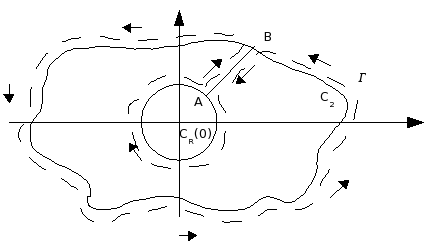
\includegraphics[height=4cm]{cauchy.png} 
\end{figure}

$$\int_{C_R(0)}\frac{dz}z=2\pi i$$
$$\int_{C_2}\frac{dz}z=?$$
Creo un circuito $\Gamma=C_2+[B,A]-C_R(0)+[A,b]$ cammino chiuso, $C^1$ a tratti, che non contiene 0 all'interno. (tratteggiato nel disegno)
\begin{align*}
	\int_\Gamma\frac{dz}z&=\int_{C_2}+\int_{[B,A]}+\int_{-C_R(0)}+\int_{[A,B]}=\\
		&=\int_{C_2}+\int_{[B,A]}-\int_{C_R(0)}-\int_{[B,A]}=0 &\mbox{per il teorema}
\end{align*}
Quindi:
$$\int_{C_2}=\int_{C_R(0)}=2\pi i$$

\newpage
\subsubsection{Circuiti omotopi}
$C_1$ e $C_2$ due circuiti di $\Omega$ $(sost(C_1)\subset\Omega)$ sono $\Omega$-\textbf{omotopi} se esiste una funzione 
$$F:[0,1]x[a,b]\to\Omega$$
continua (nelle due variabili) tale che:
\begin{itemize}
  \item $\forall \lambda \in[0,1]$, $H(\lambda,\cdot)$ \'e una parametrizzazione di un circuito in $\Omega$.
  \item $\lambda=0\Rightarrow H(0,\cdot)$ \'e una parametrizzazione di $C_1$.
  \item $\lambda=1\Rightarrow H(0,\cdot)$ \'e una parametrizzazione di $C_2$.
\end{itemize}
\begin{figure}[htbp] 
   \centering
   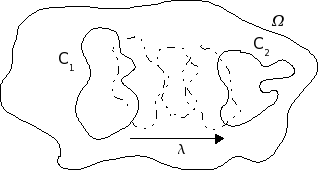
\includegraphics[height=3cm]{omotopi.png} 
\end{figure}In particolare, se ho un circuito $\Omega$-omotopo ad un punto si dice $\Omega$-omotopo a 0.
\begin{figure}[htbp] 
   \centering
   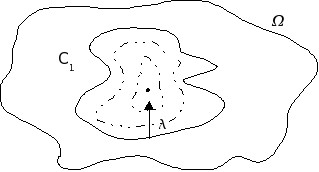
\includegraphics[height=3cm]{omotopi0.png} 
\end{figure}

\subsubsection{Teorema di Cauchy (2 versione)}
$f:\Omega\to C$, $\Omega$ aperto, $f$ olomorfa; $C_1$ e $C_2$ circuiti $\Omega$-omotopi. Allora:
$$\int_{C_1}f(z)\,dz\quad=\quad\int_{C_2}f(z)\,dz$$
In particolare, se $C$ \'e $\Omega$-omotopa a zero,
$$\int_Cf(z)\,dz=0$$

\subsubsection{Teorema di Morera}
$f:\Omega\to C$ continua\\
$\forall C$ circuito in $\Omega$ succede che se:
$$\int_Cf(z)\,dz=0$$
Allora $f$ \'e olomorfa. (Condizione sufficiente, non necessaria).\\
\\
Esempio:\\
$f(z)=\frac1z$ olomorfa in $C-\{0\}$
$$\int_{C_R(0)}\frac{dz}z=2\pi i\not= 0$$

\subsection{Sviluppi in serie}

\subsubsection{Funzione analitica}
$f:\Omega\to C$, $\Omega\subset C$ aperto\\
$f$ \'e \textbf{analitica} in $\Omega$ se \'e sviluppabile in serie di potenze di $\Omega$, cio\'e se:\\
\\
$\forall z_0 \in \Omega\quad \exists \delta>0\quad:\quad B_\delta(z_0)\subset\Omega\quad$ e $\quad\exists \{c_n\}_{n\in N}\subset C\quad$ tale che:
$$f(z)=\sum_{n=0}^{\infty}\underbrace{c_n(z-z_0)^n}_{\mbox{serie di pot. con raggio di conv.} R\geq\delta}\quad\forall z\in B_\delta(z_0)$$
Si nota che:
\begin{itemize}
  \item la serie di potenze \'e derivabile termine a termine
  \item la serie delle derivate \'e una serie con lo stesso raggio di convergenza
  \item $f$ \'e derivabile infinite volte in $B_\delta$, quindi anche in $\Omega$, quindi $f\in C^\infty$
\end{itemize}

\subsubsection{Serie di Taylor}
$f:\Omega\to C$, $\Omega$ aperto $\subset C$, $f$ analitica in $C$\\
$\forall z_0 \in \Omega\quad\exists \delta>0$ tale che
$$f(z)=\sum^{\infty}_{n=0}C_n(z-z_0)^n\quad \forall z \in B_\delta(z_0)\subset \Omega$$
serie con raggio di convergenza $R\geq\delta$, derivabile termine a termine, dalle derivate con lo stesso $R$
\begin{align*}
	f'(z)&=\sum_{n=1}^{\infty}n\cdot C_n(z-z_0)^{n-1}\quad\mbox{in }B_\delta(z_0)\\
	f''(z)&=\dots\\
	f'''(z)&=\dots\\
	\vdots&\\
	f(z_0)&=C_0\\
	f'(z_0)&=1\cdot C_1\\
	f''(z_0)&=2\cdot1\cdot C_2\\
	\vdots&\\
	f^{(n)}(z_0)&=n!\cdot C_n
\end{align*}
$$C_n=\frac{f^{(n)}(z_0)}{n!}\qquad\mbox{Coefficiente di Taylor}$$
$$f(z)=\sum_{n=0}^{\infty}\frac{f^{(n)}(z_0)}{n!}(z-z_0)^n\qquad\mbox{Serie di Taylor}$$
$f$ analitica in $\Omega$ $\Rightarrow$ $f$ sviluppabile in serie di Taylor in $\Omega$, ovvero:\\
$\forall z_0 \in\Omega\quad\exists\delta>0\quad:\quad B_\delta(z_0)\subset \Omega$
$$f(z)=\sum\mbox{Taylor}$$

\subsubsection{Serie assolutamente convergente}
$$\sum_{n=0}^{\infty}\mid C_n\mid\cdot\mid z-z_0\mid^n\qquad\mbox{\'e convergente}$$

\subsubsection{Teorema}
Serie assolutamente convergente in $B_\delta(z_0)$, $\mid z-z_0\mid<\delta$\\
$\Rightarrow$\\
Serie uniformemente convergente in $\overline{B_r(z_0)}$, $0<r<\delta$, $\mid z-z_0\mid\leq r$
$$immagine$$

\subsubsection{Formule di Cauchy}
\begin{align*}
	\int_{C_r(z_0)}\frac{f(z)}{(z-z_0)^{k+1}}\,dz&=\int_{C_r(z_0)}\frac{\sum_{n=0}^{\infty}c_n(z-z_0)^n}{(z-z_0)^{k+1}}\\
		&= \sum_{n=0}^{\infty}\int_{C_r(z_0)}c_n(z-z_0)^{n-k+1}\,dz\\
		&=\sum_{n=0}^{\infty}c_n\int_{C_r(z_0)}(z-z_0)^{n-k+1}\,dz
\end{align*}
Tutti gli integrali sono nulli a meno che l'argomento non sia pari a -1, in questo caso varr\'a $2\pi i$
$$=\sum_{n-k-1\not=1\,n=0}^{\infty}c_n\int_{C_r(z_0)}(z-z_0)^{n-k-1}+c_k\int_{}(z-z_0)^{-1}\,dz=2\pi i\cdot c_k$$
Da cui saltano fuori le formule:
\begin{align*}
	c_k&=\frac1{2\pi i}\int_{c_r(z_0)}\frac{f(z)}{(z-z_0)^{k+1}}\,dz\\
	c_n&=\frac1{2\pi i}\int_{c_r(z_0)}\frac{f(z)}{(z-z_0)^{n+1}}\,dz
\end{align*}
Ora ricavo le derivate (\textbf{formule di Cauchy}):
\begin{align*}
	f^n(z_0)&=\frac{n!}{2\pi i}\int_{C_r(z_0)}\frac{f(z)}{(z-z_0)^{n+1}}\,dz\\
	f(z_0)&=\frac1{2\pi i}\int_{C_r(z_0)}\frac{f(z)}{z-z_0}\,dz
\end{align*}
Conosco la funzione al contorno del cerchio e posso trovarmi la funzione al centro:
$$f(w)=\frac1{2\pi i}\int_{C_r(z_0)}\frac{f(z)}{z-w}\,dz\qquad\forall w\in B_r(z_0)$$
Parto dalla funzione al contorno per trovare qualsiasi punto $w$ all'interno della palla:
$$f'(w)=\frac1{2\pi i}\int_{C_r(z_0)}\frac{f(z)}{(z-w)^2}\,dz$$

\subsubsection{Teorema}
$f:\Omega\to C$, $\Omega$ aperto $\subset C$. Allora $f$ \'e olomorfa in $\Omega$ $\Leftrightarrow$ $f$ \'e analitica.\\\\
Inoltre:
$$f(z)=\sum_{n=0}^{\infty}\frac{f^{(n)}(z_0)}{n!}(z-z_0)^n\,dz\qquad\forall B_\delta(z_0)\subset\Omega$$
Nel caso reale: $f$ analitica $\stackrel{\not\Leftarrow}{\Rightarrow}$ sviluppabile in serie di potenze $\stackrel{\not\Leftarrow}{\Rightarrow}$ $f\in C^\infty$ $\stackrel{\not\Leftarrow}{\Rightarrow}$ $f$ derivabile.\\\\
Nel caso complesso: $f$ derivabile $\Leftrightarrow$ $f$ analitica ($\Leftrightarrow f\in C^\infty$)

\subsection{Singolarit\'a isolate}
$\Omega\subset C$ aperto, $z_0\in \Omega$\\\\
$f:\Omega\backslash\{z_0\}\to C$ olomorfa, $f$ \emph{non} definita in $z_0$ (\'e un punto interno, quindi esiste una palla centrata in $z_0$ nella quale $f$ \'e definita).\\\\
Allora $z_0$ \'e una \textbf{singolarit\'a isolata} per $f$.

\paragraph{Esempio}
$$f(z)=\frac1z$$
$f:C\backslash\{0\}\to C$, quindi $z_0=0$ singolarit\'a isolata

\paragraph{Esempio}
$$f(z)=\frac1{\sin z}$$
$f:C\backslash(\bigcup_{k\in z}\{k\pi\})\to C$, quindi $z=k\pi$ singolarit\'a isolate

\subsubsection{Teorema}
Dunque, ricordiamo che in assenza di singolarit\'a abbiamo che, con $f$ olomorfa in $B_\delta(z_0)\subset C$,
$$f(z)=\sum_{n=0}^{\infty}\frac{f^{(n)}(z_0)}{n!}(z-z_0)^n\qquad\forall z\in B_\delta(z_0)$$
Se invece siamo in presenza di singolarit\'a, quindi\\\\ $\Omega\subset C$ aperto, $z_0\in \Omega$ singolarit\'a isolata, $f:\Omega\backslash\{0\}\to C$ olomorfa, e
supponiamo di avere $B_R(z_0)\subset \Omega$,\\\\
Allora esiste $\{c_n\}_{n\in Z}$ tale che $\forall z\in B_R(z_0)$, con $z\not= z_0$
$$f(z)=\underbrace{\sum_{n=0}^{\infty}c_n(z-z_0)^n}_{\mbox{parte regolare}}+\underbrace{\sum_{n=1}^{\infty}c_{-n}(z-z_0)^{-n}}_{\mbox{parte singolare}} \qquad \mbox{Serie di Laurent}$$
Inoltre,
\begin{itemize}
	\item $\sum_{n=0}^{\infty}c_nw^n$ ha raggio di convergenza $\geq R$
	\item $\sum_{n=1}^{\infty}c_{-n}w^n$ ha raggio di convergenza $+\infty$
\end{itemize}
Quindi:
$$f(z)=\sum_{n=-\infty}^{+\infty}c_n(z-z_0)^n\qquad 0<\mid z-z_0\mid<R$$
$$c_n=\frac1{2\pi i}\int_{C_r(z_0)}\frac{f(z)}{(z-z_0)^{n+1}}\,dz\qquad 0<r<R\quad\forall n\in Z$$

\paragraph{Esempio}
$$f(z)=\frac1z$$ 
con $f:C\backslash\{0\}\to C$, quindi $z_0=0$ singolarit\'a isolata.\\\\
$f(z)=\sum_{n=-\infty}^{\infty}c_nz^n=z^{-1}$
\begin{itemize}
	\item $c_n=0$ $\forall n\not= -1$
	\item $c_{-1}=1$
\end{itemize}

\paragraph{Esempio}
$$f(z)=\frac1{z(1-z)}$$
definita per $z\not=0$, $z\not=-1$\\\\
Attorno a 0: 
$$f(z)=\sum_{n=-\infty}^{\infty}c_nz^n=\frac1z+\frac1{1-z}=\frac1z+\sum_{n=0}^{\infty}z^n$$
\begin{itemize}
	\item $c_n=1$ $\forall n\geq0$
	\item $c_{-1}=1$
	\item $c_n=0$ $\forall n<-1$
\end{itemize}
$\sum_{n=0}^{\infty}c_nz^n=\sum_{n=0}^{\infty}w^n$ ha raggio 1\\\\
$\sum_{n=1}^{\infty}c_{-n}z^n=w$ ha raggio $\infty$

\paragraph{Esempio}
$$f(z)=e^{\frac1z}\qquad z\not=0$$
$$f(z)=\sum_{n=-\infty}^{\infty}c_nz^n=\sum_{n=0}^{\infty}\frac{(\frac1z)^n}{n!}=\sum_{n=0}^{\infty}\frac1{n!}z^{-n}=1+\sum_{n=1}^{\infty}\frac{1}{n!}z^{-n}$$
\begin{itemize}
	\item $1$ (parte regolare): raggio $\infty$
	\item $\sum_{n=1}^{\infty}\frac{1}{n!}z^{-n}$ (parte singolare): raggio $\infty$
\end{itemize}

\subsubsection{Classificazione}
\begin{itemize}
	\item $z_0$ \'e una \textbf{singolarit\'a eliminabile} se\\\\
		$\exists f^*:\Omega\to C$ olomorfa tale che $f(z)=f^*(z)\quad\forall z\not=z_0$\\\\
		ovvero $\exists f^*(z_0)=\lim_{z\to z_0}f^*(z)=\lim_{z\to z_0}f(z)$\\\\
		$f^*(z)$, continua in $z_0$, \'e detta \emph{prolungamento olomorfo} di $f$
	\item $z_0$ \'e un \textbf{polo} se\\\\
		$\exists \lim_{z\to z_0}f(z)=\infty$ (che corrisponde a dire $\lim_{z\to z_0}\mid f(z)\mid=+\infty$)
	\item $z_0$ \'e una \textbf{singolarit\'a essenziale} in tutti gli altri casi.
\end{itemize}

\paragraph{Esempio}
$$f(z)=\frac{\sin z}z\qquad z\not=0$$
$$f(z)=\frac1z\sum_{k=0}^{\infty}(-1)^k\frac{z^{2k+1}}{(2k+1)!}=\sum_{k=0}^{\infty}(-1)^k\frac{z^{2k}}{(2k+1)!}:=f^*(z)$$
Quindi $z_0=0$ \'e una singolarit\'a eliminabile.

\paragraph{Esempio}
$$f(z)=\frac1{z^m}\qquad m\geq1\quad z_0=0$$ 
$$\lim_{z\to0}\mid\frac1{z^m}\mid=\lim_{\mid z\mid\to0}\frac1{\mid z\mid^m}=\infty$$
Quindi $z_0=0$ \'e un polo.

\paragraph{Esempio}
$$f(z)=e^{\frac1z}\qquad z_0=0$$
Proviamo a studiare il limite sull'asse reale: $z=x\in R$
\begin{itemize}
	\item $\lim_{x\to0^-}e^{\frac1x}=0$ (quindi non \'e un polo)\\
	\item $\lim_{x\to0^+}e^{\frac1x}=\infty$ (diversa da prima, quindi non \'e una singolarit\'a eliminabile)
\end{itemize}
Quindi $z_0$ \'e una singolarit\'a essenziale.

\subsubsection{Teorema}
$f:\Omega\backslash\{z_0\}\to C$, $z_0$ singolarit\'a isolata.\\\\
se $\exists\delta>0\quad:\quad f$ \'e limitata in $B_\delta(z_0)\subset C$\\\\
Allora $z_0$ \'e una singolarit\'a eliminabile.\\\\
(ovvero se $\exists\delta>0$, $M>0\quad:\quad\mid f(z)\mid \leq M\quad\forall z\in B_\delta(z_0)$)\\\\\\
Da qui deriva che, se $\exists$ finito $\lim_{z\to z_0}$, allora $f$ \'e limitata in $B_\delta(z_0)$ con $\delta$ opportuno.\\\\
$z_0$ singolarit\'a eliminabile $\Leftrightarrow$ $\exists \lim_{z\to z_0}f(z)=f^*(z_0)$

\subsubsection{Classificazione (ai limiti)}
\begin{itemize}
	\item $z_0$ \textbf{singolarit\'a eliminabile} se 
		$$\exists \mbox{ finito } \lim_{z\to z_0}f(z)$$
	\item $z_0$ \textbf{polo} se 
		$$\exists \lim_{z\to z_0}f(z)=\infty$$
	\item $z_0$ \textbf{singolarit\'a essenziale} se
		$$\not\exists \lim_{z\to z_0} f(z)$$
\end{itemize}

\subsubsection{Teorema}
$z_0$ polo per $f$. Allora $\exists$ un unico $n_0\in N\geq1$ tale che:
$$\exists \mbox{ finito } \lim_{z\to z_0}(z-z_0)^{n_0}f(z)\not=0$$
ovvero
$$f(z)\approx \frac1{(z-z_0)^{n_0}}$$
$n_0$ \'e detto \textbf{ordine del polo}.

\subsubsection{Classificazione (alla serie di Laurent)}
\begin{itemize}
	\item $z_0$ \'e \textbf{singolarit\'a eliminabile} se e solo se la sua serie di Laurent ha solo parte regolare.
		$$f(z)=\sum_{n=0}^{\infty}c_n(z-z_0)^n\qquad c_n=0\forall n\leq 1$$
	\item $z_0$ \'e un \textbf{polo} se e solo se la parte singolare della sua serie di Laurent ha solo un numero finito di termini.
		$$f(z)=\sum_{n=0}^{\infty}c_n(z-z_0)^n+\sum_{n=1}^{n_0}c_{-n}(z-z_0)^{-n}\qquad c_{-n_0}\not=0$$
		$n_0$ ordine del polo.
	\item $z_0$ \'e \textbf{singolarit\'a essenziale} se e solo se la parte singolare della sua serie di Laurent ha un numero infinito di termini.
\end{itemize}

\paragraph{Esempio}
$$f(z)=\frac{\sin z}z=\sum_{k=0}^{\infty}(-1)^k\frac{z^{2k}}{(2k+1)!}$$
(ha solo parte regolare, quindi \'e una singolarit\'a eliminabile)
$$f(z)=\frac1{z^m}\qquad \lim_{z\to z_0}z^m\frac1{z^m}\not=0$$
(quindi $z_0=0$ \'e un polo di ordine m).
$$f(z)=e^{\frac1z}=\sum_{m=1}^{\infty}\frac1{m!}z^{-m}$$
(la parte singolare ha $\infty$ termini, quindi \'e una singolarit\'a essenziale)

\subsection{Residui}
Dunque, sappiamo che:
$$f(z)=\sum_{n=-\infty}^{\infty}c_n(z-z_0)^n\qquad 0<\mid z-z_0 \mid<R$$
$$c_n=\frac1{2\pi i}\int_{C_r(z_0)}\frac{f(z)}{(z-z_0)^{n+1}}\,dz\qquad0<r<R$$
A partire da qui, definiamo \textbf{residuo} di $f$ in $z_0$
$$C^{-1}=res(f,z_0)=\frac1{2\pi i}\int_{C_r(z_0)}f(z)\,dz$$

\paragraph{Esempio}
$z_0$ singolarit\'a eliminabile.
$$f(z)=\sum_{n=0}^{\infty}c_n(z-z_0)^n\qquad c_n=0\forall n\leq1$$
quindi $res(f,z_0)=0$

\paragraph{Esempio}
$$f(z)=\frac1z\qquad c_n=0\forall n\not=1\quad c_{-1}=1$$
quindi $res(\frac1z,0)=1$

\paragraph{Esempio}
\begin{align*}
	f(z)&=\frac{\sin z}{z^3}&\forall z\not=0\quad z_0=0\\
		&=\frac1{z^3}\sum_{k=0}^{\infty}(-1)^k\frac{z^{2k+1}}{(2k+1)!}=\\
		&=\frac1{z^3}\{z-\frac{z^3}{3!}+\frac{z^5}{5!}+\dots\}=\\
		&=\frac1{z^2}-\frac1{3!}+\frac{z^2}{5!}-\frac{z^4}{7!}+\dots
\end{align*}
$c_{-1}=0$ quindi $res(f,0)=0$

\subsubsection{Calcolo residui}
Supponiamo di avere un polo di ordine $\leq3$
$$f(z)=c_{-3}(z-z_0)^{-3}+c_{-2}(z-z_0)^{-2}+c_{-1}(z-z_0)^{-1}+c_0+\dots$$
Se l'ordine del polo \'e 3, allora $c_{-3}\not=0$\\
Creiamo la funzione:
$$g(z)=(z-z_0)^3f(z)=c_{-3}+c_{-2}(z-z_0)+c_{-1}(z-z_0)^2+\dots$$
Funzione analitica, quindi somma di serie di potenze, quindi la serie di Taylor di $g$ centrata in $z_0$ \'e:
$$=g(z_0)+g'(z_0)(z-z_0)+\underbrace{\frac{g''(z_0)}{2!}(z-z_0)^2}_{\mbox{residuo}}+\dots$$
Quindi:
$$c_{-1}=\frac{g''(z_0)}{2!}=\frac1{2!}\frac{d^2}{dz^2}\Bigr( (z-z_0)^3f(z) \Bigr)\mid_{z=z_0}$$
Poich\'e $f(z_0)$ non \'e definita
$$=\frac1{2!}\lim_{z\to z_0}\frac{d^2}{dz^2}\Bigr( (z-z_0)^3f(z) \Bigr)$$
Quindi, se ho un polo di ordine $\leq n$:
$$res(f,z_0)=\frac1{(n-1)!}\lim_{z\to z_0}\frac{d^{n-1}}{dz^{n-1}}\Bigr( (z-z_0)^nf(z) \Bigr)$$

\paragraph{Esempio}
$$f(z)=\frac{\sin z}{z^3}\qquad z=0\mbox{ polo di 2 ordine}$$
$$res(f,0)=1\cdot\lim_{z\to 0}\frac d{dz}(z-z_0)^2f(z)=\lim_{z\to0}\frac d{dz}(z^2\frac{\sin z}{z^3})=\lim_{z\to 0}\frac{z\cos z-\sin z}{z^2}$$
\begin{itemize}
	\item $\cos(z)=1-\frac{z^2}{2!}+\frac{z^4}{4!}+\dots=1-\frac{z^2}{2!}+o(z^3)$
	\item $\sin(z)=z-\frac{z^3}{3!}+\frac{z^5}{5!}+\dots=z+o(z^2)$
\end{itemize}
$$=\lim_{z\to0}\frac{z(1-\frac{z^2}{2!}+o(z^3))-(z+o(z^2))}{z^2}=\lim_{z\to0}\frac{o(z^2)}{z^2}=0$$

\paragraph{Esempio}
$$f(z)=\frac{e^\frac1z}{1-z}$$
\begin{itemize}
  \item $z_0=0$ singolarit\'a essenziale
  \item $z_1=1$ polo di ordine 1
\end{itemize}
$$res(f,1)=\frac1{0!}\lim_{z\to1}\frac{d^0}{dz^0}\Bigr( (z-1)^1\frac{e^\frac1z}{1-z} \Bigr)=\lim_{z\to1}(-e^\frac1z)=-e$$
\'E stato facile, poich\'e sapevo l'ordine del polo. Se non l'avessi conosciuto a priori i conti sarebbero stati molto pi\'u complessi.
$$res(f=0)=?$$
(non posso usare la formula semplificata per i poli, devo trovare lo sviluppo di Laurent)
\begin{align*}
	f(z)&=e^\frac1z\frac1{1-z}=\\
		&=\sum_{n=0}^{\infty}\frac{\Bigr(\frac1z\Bigr)^n}{n!}\cdot\sum_{k=0}^{\infty}z^k=\\
		&=\Bigr( 1+\frac{z^{-1}}{1!}+\frac{z^{-1}}{2!}+\dots \Bigr)\cdot\Bigr( 1+z+z^2+z^3+\dots \Bigr)=\\
		&=\Bigr( 1+z+z^2+z^3+\dots \Bigr)+\frac{z^{-1}}{1!}\cdot\Bigr( 1+z+z^2+\dots \Bigr)+\frac{z^{-2}}{2!}\cdot\Bigr( 1+z+z^2+\dots \Bigr)=\\
		&=1+1+1+\dots+\frac{z^{-1}}{1!}+\frac{z^{-1}}{1!}+\frac{z^{-1}}{1!}+\dots=\\
		&=\sum_{n=0}^{\infty}\sum_{k=0}^{\infty}\frac{z^{-n}}{n!}z^k&\mbox{prod. alla Cauchy}
\end{align*}
Poich\'e la prima serie converge $\forall z \not=0$ e la seconda per $\mid z\mid <1$,
$$f(z)=\sum_{n,k=0}^{\infty}\frac1{n!}z^{-n+k}$$
$$res(f,0)=c_{-1}=\sum_{\stackrel{n,k=0}{-n+k=-1}}^{\infty}\frac1{n!}=\sum_{n=1}^{\infty}\frac1{n!}=e-1\qquad \Bigr(e=\sum_{n=0}^{\infty}\frac1{n!}\Bigr)$$

\subsubsection{Teorema (prodotto alla Cauchy)}
$\sum_{n=0}^{\infty}a_nz^n$, $\sum_{n=0}^{\infty}b_nw^n$ entrambe assolutamente convergenti. Allora:
$$\Bigr( \sum_{n=0}^{\infty}a_nz^n \Bigr)\cdot\Bigr(\sum_{k=0}^{\infty} b_kw^k \Bigr)=\sum_{n=0}^{\infty}\sum_{k=0}^{\infty}a_nb_kz^nw^k$$

\subsubsection{Teorema dei residui}
$\Omega \subseteq C$ aperto, $C$ circuito $\Omega$-omotopo a 0\\\\
$z_1,z_2,\dots,z_n$ interni a $C$, $f:\Omega\backslash\{z_1,\dots,z_n\}\to C$ olomorfa\\\\
Allora:
$$\int_Cf(z)\,dz=2\pi i\Bigr(res(f,z_1)+\dots+res(f,z_n)\Bigr)$$
Infatti, nel caso di unica singolarit\'a abbiamo:
$$res(f,z_0)=c_{-1}=\frac1{2\pi i}\int_{C_r(z_0)}f(z)\,dz$$

\newpage

\paragraph{Esempio}
$$\int_{C_2(0)}\frac1{z^4-8z^2-9}\,dz=I$$
$z^4-8z^2-9=(z^2-9)(z^2+1)=0\quad\Leftrightarrow\quad \underbrace{z=\pm3, z=\pm i}_{\mbox{4 poli del 1 ordine}}$

\begin{figure}[htbp] 
   \centering
   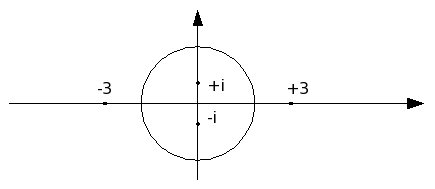
\includegraphics[height=3cm]{esthres.png} 
 \end{figure}

\noindent Si nota che i punti interni alla circonferenza sono solo $\pm i$, quindi:
$$I=2\pi i\left[ res(f,1)+res(f,-i) \right]$$
Si calcolano i residui:
\begin{align*}
	res(f,i)&=\lim_{z\to i}\frac1{0!}\frac{d^0}{dz^0}\Bigr[ (z-1)f(z) \Bigr]=\\
		&=\lim_{z\to1}\frac{(z-i)}{(z-i)(z+1)(z-3)(z+3)}=\\
		&=\frac1{2i(i+3)(i-3)}\\
	res(f,-1)&=\lim_{z\to-i}\frac1{0!}\frac{d^0}{dz^0}\Bigr[ (z+i)f(z) \Bigr]=\\
		&=\frac1{-2i(-i+3)(-i3)}
\end{align*}
Da cui:
$$res(f,i)+res(f,-i)=0\quad\Leftrightarrow \quad I=0$$

\paragraph{Esempio}
$$I=\int_{-\infty}^{+\infty}\frac1{1+x^2}\,dx$$
Il metodo sempilce per calcolare l'integrale \'e:
$$I=\lim_{R\to\infty}\int_{-R}^R\frac{dx}{1+x^2}=\lim_{R\to\infty}\arctan x\mid_{-R}^{R}=\lim_{R\to\infty}2\arctan R=2\frac\pi2=\pi$$
Oppure si pu\'o fare con il metodo visto prima. Parametrizziamo la funzione $f(z)$:\\\\
$f(z)=\frac1{1+z^2}$, $f:C\backslash\{\pm i\}\to C$ olomorfa\\\\
E poi costruiamo il seguente circuito chiuso:
\begin{figure}[htbp] 
   \centering
   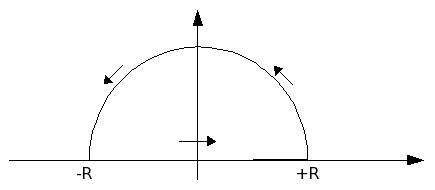
\includegraphics[height=3cm]{es2thres.png} 
 \end{figure}
$$C=C_R^++[-R,R]$$
$$\int_Cf(z)\,dz=\int_{C_R^+(0)}f(z)\,dz+\int_{-R}^Rf(x)\,dx=2\pi i\cdot res(f,i)$$
$$=2\pi i\cdot\lim_{z\to i}(z-i)f(z)=2\pi i\lim_{z\to i}\frac{z-i}{(z+i)(z-i)}=2\pi i\frac1{2i}=\pi$$
A questo punto, dobbiamo calcolare il valore dell'integrale:
$$\int_{C_R^+(0)}\frac1{1+z^2}\,dz$$
Che, parametrizzando la curva, diventa:
\begin{itemize}
	\item $z=r(t)=Re^{it}$, con $t\in[0,\pi]$
	\item $dz=r'(t)=Re^{it}i\,dt$
\end{itemize}
$$\int_0^\pi\frac{Rie^{it}}{1+R^2e^{2it}}\,dt$$
che in modulo pu\'o essere maggiorato da:
$$\leq\int_0^\pi\frac R{R^2-1}\,dt=\frac{R\pi}{R^2-1}\,dt\to0\quad \mbox{per }R\to\infty$$
Quindi, essendo nullo quest'ultimo integrale, risulta che:
$$0+\int_{-R}^Rf(x)\,dx=\pi$$

\paragraph{Esempio}
$$\int_{-\infty}^{\infty}\frac{\sin x}x\,x$$
Definisco $f(z)$:\\\\
$f(z)=\frac{e^{iz}}{z}$, con $x\in R$, $f:C\backslash\{0\}\to C$ olomorfa\\\\
in modo tale che l'integrale risulta:
$$=\lim_{\stackrel{R\to+\infty}{\varepsilon\to0^+}}\int_{\varepsilon<\mid x\mid \leq R}\frac{\sin x}{x}\,dx$$
Construisco un percorso:
\begin{figure}[htbp] 
   \centering
   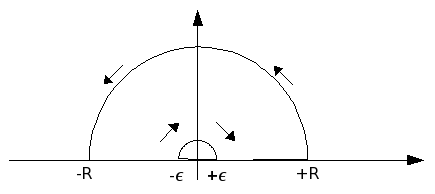
\includegraphics[height=3cm]{es3thres.png} 
 \end{figure}
$$C=C_R^+(0)+[-R,-\varepsilon]-C_\varepsilon^+(0)+[\varepsilon,R]$$
Poich\'e non ci sono singolarit\'a in $C$,
$$\int_Cf(z)\,dz=0=\int_{C_R^+(0)}+\int_{-R}^{-\varepsilon}+\int_{C_\varepsilon^+(0)}+\int_\varepsilon^R$$
$$\lim_{R\to+\infty}\int_{C_R^+(0)}-\lim_{\varepsilon\to0}\int_{C_\varepsilon^+(0)}+\underbrace{\lim_{\stackrel{R\to+\infty}{\varepsilon\to0}}\Bigr[ \int_{-R}^{-\varepsilon}+\int_{\varepsilon}^{R} \Bigr]}_{\int_{-\infty}^{\infty}\frac{e^{ix}}{x}\,dx}=0$$
Calcoliamo il valore dei singoli integrali:
\begin{align*}
	\lim_{R\to\infty}\int_{C_R^+(0)}\frac{e^{iz}}z&=\int_0^\pi\frac{e^{iRe^{it}}}{Re^{it}}Rie^{it}\,dt=\\
		&=\int_0^\pi ie^{iRe^{it}}\,dt
		&\mbox{che in modulo pu\'o essere maggiorato da}\\
		&\leq\int_0^\pi\mid e^{iRe^{it}}\mid\,dt\\
		&=\int_0^\pi \mid e^{iR(\cos t+i\sin t)}\mid\,dt\\
		&=\int_0^\pi\mid\underbrace{e^{iR\cos t}}_{\mbox{modulo 1}}\cdot e^{-R\sin t}\mid\,dt\\
		&=\int_0^\pi e^{-R\sin t}\,dt\to0\\\\
	\lim_{\varepsilon\to0}\int_{C_\varepsilon^+(0)}\frac{e^{iz}}{z}\,dz&=\lim_{\varepsilon\to0}\int_0^\pi ie^{i\varepsilon e^{it}}\,dt=\int_0^\pi i\,dt=\pi i
\end{align*}
Quindi;
$$0-\pi i+\int_{-\infty}^{\infty}\frac{e^{ix}}x\,dx=0$$
$$\frac{e^{ix}}x\,dx=\pi i=\int_{-\infty}^{+\infty}\frac{\cos x+i\sin x}x\,dx=\underbrace{\int\frac{\cos x}x}_{J}+\underbrace{i\int\frac{\sin x}z}_I=\pi i$$
$$J+iI=\pi i \quad \Rightarrow\quad J=0\quad I=\int_{-\infty}^{\infty}\frac{\sin x}x\,x=\pi$$

\newpage

\subsection{Funzioni Polidrome}

\subsubsection{Logaritmo}
Logaritmo: $z\to w$ funzione inversa di $z=e^w$: $w\to z$ (esponenziale).\\\\
Dato $z\not=0$, $z=\rho e^{i\theta}$, $\rho>0$, definiamo:
$$w=\log\rho+i(\theta+2\pi k)$$
per ogni $k\in z$. A questo punto, verifichiamo inserendo il $w$ appena definito nell'esponenziale:
$$e^w=e^{\log \rho+i(\theta+2\pi k)}=e^{\log \rho}\cdot e^{i(\theta+2\pi k)}=\rho e^{i\theta}\underbrace{e^{i2\pi k}}_{1}=\rho e^{i\theta}=z$$
per ogni $k\in z$. Quindi, abbiamo verificato che:
$$e^w=z\quad\forall k$$
ovvero per infiniti valori di w, in cui la fase varia di $k2\pi$. Abbiamo realizzato una funzione a pi\'u valori, ovvero \textbf{multivoca}. Definiamo:
$$arg(z)=\Bigr\{ \theta\in R\quad:\quad z=\mid z\mid e^{i\theta} \Bigr\}$$
$$\log(z)=\Bigr\{ \log\mid z\mid +i\theta, \quad\theta\in arg(z) \Bigr\}$$
La funzione \'e detta \textbf{funzione con $\infty$ branche}, ciascuna delle quali impedisce un giro completo attorno all'origine. Ad esempio, sono equivalenti:
\begin{align*}
	f_1(z)&=\log\mid z\mid+i\theta&\theta\in]0,2\pi[\\
	f_2(z)&=\log\mid z\mid+i\theta&\theta\in\Bigr]-\frac\pi2, \frac32\pi\Bigr[\\
	f_3(z)&=\log\mid z\mid+i\theta&\theta\in\Bigr]-\pi,\pi\Bigr[\\
\end{align*}
$z=0$ \'e detto \textbf{punto di diramazione}.

\subsubsection{Radice}
La radice \'e funzione inversa della potenza $w\to z=w^n$, quindi $w\sim\sqrt[n]{z}$\\\\
Scrivendo $z=\rho e^{i\theta}$, immaginiamo un $w_k$:
$$w_k=\sqrt[n]{\rho}\cdot e^{i\frac{\theta+2k\pi}n}$$
Verifichiamo inserendo $w_k$ nella potenza:
$$w_k^n=\Bigr( \sqrt[n]{\rho}\cdot e^{i\frac{\theta+2k\pi}n} \Bigr)^n=\rho\cdot e^{i(\theta+2\pi i)}=\rho\cdot e^{i\theta}\quad\forall k\in Z$$ 
Quindi definiamo la radice di $z$ come:
$$\sqrt[n]{z}=\Bigr\{ \sqrt[n]{\rho}\cdot e^{i\frac\theta n}\quad\theta\in arg(z) \Bigr\}$$
Come prima, abbiamo una suddivisione in infinite branche per poter avere una funzione univoca (olomorfa). $z_0=0$ \'e ancora detto \textbf{punto di diramazione}.

\paragraph{Esempio}
$$\int_{-\infty}^{+\infty}\frac{\sqrt{x}}{1+x^2}$$
Definiamo:
$$f(z)=\frac{\sqrt{z}}{z^2+1}$$
Con:
\begin{itemize}
  \item $z=0$ punto di diramazione della radice
  \item $z=\pm i$ poli di ordine 1
\end{itemize}
Scelgo la branca che esclude il semiasse positivo:
$$\sqrt{z}=\sqrt{\mid z\mid}e^{i\frac\theta2}\qquad\theta\in]0,2\pi[$$
\begin{figure}[htbp] 
   \centering
   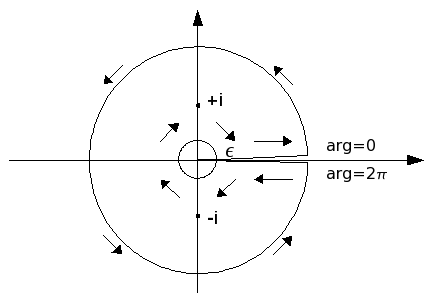
\includegraphics[height=4cm]{esradice.png} 
 \end{figure}
$$C=C_R(0)+[R,\varepsilon]-C_\varepsilon(0)+[\varepsilon,R]$$
$$\int_Cf(z)\,dz=2\pi i[res(f,i)+res(f,-1)]$$
Quindi posso ridurre l'integrale al calcolo dei residui dei due poli:
\begin{align*}
	res(f,i)&=\lim_{z\to i}(z-i)f(z)=\\
		&=\lim_{z\to i}(z-i)\frac{\sqrt z}{(z+i)(z-i)}=\frac{\sqrt i}{2i}=\frac{\sqrt1\cdot e^{i\frac\pi{2\cdot2}}}{2i}=
		&\quad\Bigr( \sqrt z=\sqrt{\mid z\mid}\cdot e^{i\frac\theta2} \Bigr)\\
		&=\frac{e^{i\frac\pi4}}{2i}=\frac{\cos \frac\pi4+i\sin\frac\pi4}{2i}=\frac{\sqrt2}{4i}+\frac{\sqrt2}{4}\\
		\\
	res(f,-i)&=\dots=\frac{\sqrt2}{4i}-\frac{\sqrt2}{4}
\end{align*}
Quindi:
$$\int_{-\infty}^{+\infty}\frac{\sqrt{x}}{1+x^2}=2\pi i\Bigr(\frac{\sqrt2}{4i}+\frac{\sqrt2}{4}+\frac{\sqrt2}{4i}-\frac{\sqrt2}{4} \Bigr)=\pi\sqrt2$$

\subsection{Integrali di Lebesgue}
Metodo pi\'u potente dei precedenti per il calcolo di integrali e funzioni non integrabili normalmente.
\subsubsection{Misura}
\begin{itemize}
  \item A partire da $I$ intervallo limitato in $R$, definiamo \textbf{misura} di $I=m(I)=mis(I)=\mid I\mid=b-a$\\Esempi:
  	\begin{itemize}
	  \item $I=[a,b[$ (estremo mancante)
	  \item $I=\{a\}$ punto, quindi $\mid I\mid =0$
	\end{itemize}
  \item $R$ \textbf{rettangolo} in $R^n$
  	\begin{itemize}
	  \item $R=I_1\times I_2\times I_3\times\dots\times I_n$
	  \item $mis(R)=\mid I_1\mid\cdot\mid I_2\mid\cdot\dots\cdot\mid I_n\mid =\prod_{k=1}^n\mid I_k\mid$
	\end{itemize}
  \item $P$ \textbf{plurirettangolo} 
	\begin{itemize}
	  \item $P=\bigcup_{k=1}^{m}R_k$
	  \item $mis(P)=\sum_{k=1}^mmis(R_k)$ (se gli $R_k$ non hanno interni in comune)
	\end{itemize} 
\end{itemize}
Inoltre, $A\subset R^n$ ha \textbf{misura nulla} ($mis(A)=0$) se:\\
$\forall \varepsilon>0\quad\exists\{R_k\}_{k\geq1}$ tale che:
\begin{itemize}
	\item $A\subset \bigcup_{k=1}^{\infty}R_k$
	\item $\sum_{k=1}^\infty m(R_k)<\varepsilon$
\end{itemize}

\paragraph{Esempio}
$n=2$, $R=[a,b]\times \{c\}$
\begin{figure}[htbp] 
   \centering
   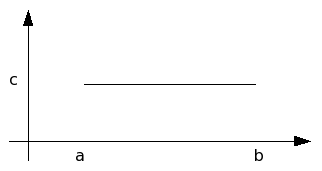
\includegraphics[height=3cm]{segmento.png} 
 \end{figure}
$$\forall \varepsilon>0\quad\mid R_\varepsilon\mid=(b-a)\cdot\frac\varepsilon{2(b-a)}=\frac\varepsilon2<\varepsilon$$

\subsubsection{Proposizione Quasi Vera (?!?)}
Una proposizione $P(x)$ \'e vera per quasi ogni $x$ ($q.o.x$) se:
$$mis\Bigr( \Bigr\{ x\quad:\quad P(x)\mbox{ \'e falsa} \Bigr\} \Bigr)=0$$

\paragraph{Esempi:}
\begin{itemize}
  \item $u,v$ due funzioni.\\
  	$u=v$ per q.o.x se $m(\{u:u(x)\not=v(x)\})=0$
  \item $u(x)= 1$ se $x\in Q$, $0$ se $x\in R\backslash Q$\\
  	$\{x\in R:u(x)\not=0\}=\{x\in R:u(x)=1\}=Q$\\
	$mis(Q)=0\longrightarrow u(x)=0$ q.o.x	
\end{itemize}

\subsubsection{Successione di Cauchy}
$\{a_n\}_{n\in N}\subset R$ \'e una \textbf{successione di Cauchy} se:\\\\
$\forall \varepsilon>0\quad\exists n_0\in N\quad:\quad\forall n,m\geq n_0 \quad \mid a_n-a_m\mid <\varepsilon$

\subsubsection{Convergenza}
$\{a_n\}_{n\in N}$ \'e \textbf{convergente} a L se:\\\\
$\forall \varepsilon>0\quad \exists n_i\in N\quad:\quad\forall n\geq n_i \quad \mid a_n-L\mid<\varepsilon\quad e\quad\lim_{n\to\infty}a_n=L$\\
\\
Inoltre, accade che se $\{a_n\}$ \'e una successione convergente, allora \'e una successione di Cauchy.\\
\\
Dimostrazione:\\
$\forall \varepsilon>0\quad\exists n_1\quad:\quad\forall n\geq n_1\quad\mid a_n-L\mid<\frac\varepsilon2$\\\\
$\forall n,m\geq n\quad\mid a_n-a_m\mid=\mid a_n-L-(a_m-L)\mid\leq\mid a_n-L\mid+\mid a_m-L\mid<\frac\varepsilon2+\frac\varepsilon2<\varepsilon$

\subsubsection{Teorema}
$\{a_n\}_{n\in N}\subset R$ successione di Cauchy \'e una successione convergente.
$$\mbox{convergente} \stackrel{\mbox{(in R)}}{\Longleftrightarrow}\mbox{Cauchy}$$

\paragraph{Esempio}
$\sqrt2\in R\backslash Q$ numero irrazionale\\
$\{x_k\}\in Q$, $x\to\sqrt2$ per $k\to\infty$\\
$\{x_k\}$ \'e convergente in $R$ $\Rightarrow$ Cauchy in $R$ $\Rightarrow$ Cauchy in $Q$, ma non \'e convergente in $Q$ poich\'e converge a un numero irrazionale!

\subsubsection{Funzione Caratteristica}
$A\in R^n$ \'e \textbf{funzione caratteristica} dell'insieme A:
\begin{align*}
	\chi_A(x)&=1\quad x=A\\
		&=0\quad x\not=A
\end{align*}

\paragraph{Esempio}
\begin{align*}
	u(x)&=1\quad x\in Q&u=\chi Q\\
		&=0\quad x\not\in Q
\end{align*}

\subsubsection{Funzione a Scala}
$u:R^n\to C$ \'e una \textbf{funzione a scala} 
$$u(x)=\sum_{k=1}^{m}C_k\cdot\chi_{R_k}(x)$$
con $R_k$ rettangoli, $C_k \in C$
$$IMMAGINE$$

\subsubsection{Integrale di funzione a scala}
$$\int_{R^n}u=\int_{R^n}u(x)\,dx=\sum_{k=1}^{m}C_k\cdot m(R_k)$$

\subsubsection{Integrabilit\'a secondo Lebesgue}
$u:R\to C$ \'e integrabile secondo Lebesgue (o sommabile) se:
\begin{enumerate}
	\item $u$ \'e misurabile, ovvero esiste una successione $\{u_k\}_{k\in N}$ di funzioni a scala tale che:
	$$u(x)=\lim_{k\to\infty}u_k(x)\quad q.o.x$$
	\item $\forall \varepsilon>0\quad\exists k_0\in N$ tale che $\forall k,k'\geq k_0$ si ha che
	$$\int_{R^n}\mid u_k(x)-u_{k'}(x)\mid\,dx<\varepsilon$$
\end{enumerate}

\paragraph{Osservazione}
La successione numerica $\{\int_{R^n} u_k(x)\,dx\}$ \'e una successione di Cauchy.
$$\Big| \int_{R^n}u_k(x)\,dx-\int_{R^n}u_{k'}(x) \Big|=\Big|\int_{R^n}[u_k(x)-u_{k'}(x)]\,dx\Big|\leq$$
$$\leq\int_{R^n}|u_k(x)-u_{k'}(x)|\,dx<\varepsilon\quad\forall k,k'\geq k_0$$
Quindi la successione $\{\int_{R^n}u_k(x)\,dx\}$ \'e convergente in $C$.

\subsubsection{Integrale secondo Lebesgue}
L'integrale secondo Lebesgue di  $u$ \'e:
$$\int_{R^n}u\,dx=\int_{R^n}u(x)\,dx=\lim_{k\to\infty}\int_{R^n}u_k(x)\,dx$$

\paragraph{Proposizione}
$u$ misurabile \'e integrabile se esiste una funzione $\varphi$ integrabile tale che
$$|u(x)|\leq\varphi(x)\quad q.o.x$$
Quindi $u$ \'e integrabile se e solo se $|u|$ \'e integrabile. Si dimostra semplicemente sapendo che:
\begin{itemize}
	\item $u$ integrabile $\Rightarrow$ $|u|$ integrabile. (dalla definizione)
	\item $|u|$ integrabile; basta scegliere $\varphi=|u|$ e applicare la proposizione.
\end{itemize}

\subsubsection{Insieme misurabile}
Un insieme A \'e misurabile se $\chi_A$ \'e una funzione misurabile\\\\
ovvero se esiste una successione di funzioni a scala $\{u_k\}$ tale che $u_k\to\chi_A(x)$ q.o.x

\subsubsection{Insieme di misura finita}
Se $\chi_A$ \'e integrabile, si dice che $A$ \'e un \textbf{insieme di misura finita}.
$$|A|=m(A)=mis(A)=\int_{R^n}\chi_A(x)\,dx$$
Se $\chi_A$ non \'e integrabile, si dice che $A$ ha\textbf{ misura infinita}.
$$IMMAGINE$$

\paragraph{Esempio}
$mis(R^n)=\infty$

\subsubsection{Integrabilit\'a secondo Lebesgue su insieme finito}
$u:A\to C$, $A$ misurabile $\subset R$\\\\
$u$ \'e integrabile su $A$ (secondo Lebesgue) se
$$
	\tilde u(x)=\bigg\{ 
	\begin{array}{rl}
		u(x)&x\in A\\
		0&x\not\in A
	\end{array}	
$$
se $\tilde u$ \'e integrabile su $R^n$. (sono tornato alla definizione di integrale su tutto $R^n$).

\subsubsection{Confronto con l'integrale secondo Riemann}
Data $u:R^n\to C$ limitata, $u$ nulla fuori da un insieme limitato, integrabile secondo Riemann.\\\\
Allora $u$ \'e integrabile secondo Lebesgue e vale:
$$\int_Lu=\int_Ru$$
Se $u$ \'e integrabile secondo Lebesgue, allora $|u|$ \'e integrabile secondo Lebesgue.\\\\
Dunque l'integrale improprio secondo Riemann esiste solo se questo \'e assolutamente convergente.\\\\
Possono esistere funzioni con integrale improprio ma non l'integrale secondo Lebesgue.

\paragraph{Esempio}
Esiste l'integrale improprio 
$$\int_R \frac{\sin x}x\,dx=\pi$$
ma non l'integrale secondo Lebesgue:
$$\int_R\Big| \frac{\sin x}x \Big|\,dx=+\infty$$

\subsubsection{Teorema di Lebesgue della convergenza dominata}
\begin{itemize}
	\item $u_k:A\to C$, $A$ misurabile, $u_k$ funzioni integrabili.
	\item $u_k\to u$ q.o.$x\in A$
	\item $\exists \varphi\geq0$ integrabile su A tale che $|u_k(x)|\leq\varphi(x)$ q.o.x, $\forall k$
\end{itemize}
Allora:
\begin{enumerate}
	\item $u$ \'e integrabile.
	\item $\int_Au_k(x)\,dx\to\int_Au(x)\,dx$
\end{enumerate}

\subsubsection{Esempio: confronto con la teoria classica (di Riemann)}
La teoria classica prevede che:
\begin{itemize}
	\item $f_n:[a,b]\to R$ integrabili
	\item $f_n\to f$ \textbf{uniformemente} in $[a,b]$
\end{itemize}
in tal caso:
\begin{enumerate}
	\item $f$ integrabile
	\item $\int_a^bf_n(x)\,dx\to\int_a^bf(x)\,dx$
\end{enumerate}
Quindi, ad esempio, per risolvere l'integrale:
$$\lim_{k\to \infty}\int_0^\pi e^{-k\sin x}\,dx$$
Si studia $u_k(x)=e^{-k\sin x}$ che \'e continua in $[0,\pi]$. Per\'o:
$$
	u(x)=\lim_{k\to\infty}e^{-k\sin x}=\Big\{
	\begin{array}{rl}
		1&x=0,\pi\\0&x\in]0,\pi[
	\end{array}
$$
Quindi non c'\'e convergenza uniforme, e la teoria classica non \'e dunque applicabile. \\\\
Invece, con Lebesgue, noto che $|u_k(x)|\leq1\quad\forall x,\forall k$. Scelgo dunque $\varphi(x)=1$, integrabile su $[0,\pi]$.
$$\int_0^\pi e^{-k\sin x}\,dx=\int_0^\pi u(x)\,dx$$
$$u(x)=0\quad q.o.x\quad\Rightarrow\quad\int_0^\pi u(x)\,dx=0$$
Ovvero, con Lebesgue le discontinuit\'a che costituiscono insiemi di misura nulla (come i due estremi dell'esempio) non influiscono sul risultato.

\paragraph{Corollario}
$$\int_A|u_k(x)-u(x)|\,dx\to 0\quad\mbox{per }k\to\infty$$
Si dimostra a partire dal fatto che $u$ integrabile $\Rightarrow$ $|u|$ integrabile:
$$|u_k(x)-u(x)|\to 0\quad q.o.x$$
$$|u_k(x)-u(x)|\leq|u_k(x)|+|u(x)|\leq\varphi(x)+|u(x)|\quad\forall k, q.o.x$$
$$\int_A|u_k(x)-u(x)|\,dx\to 0$$

%-------------------------------------------------------------------------

\section{Spazi vettoriali normati}

V \'e \textbf{spazio vettoriale} su $C$ (o $R$) se\\\\
$\forall u,v\in V\quad\forall \lambda,\mu\in C\quad\mbox{vale che}\quad\lambda\cdot u+\mu\cdot v\in V$

\subsection{Norma}
$||\cdot||:V\to R$ \'e una \textbf{norma} se:
\begin{enumerate}
	\item $||u||\geq0$ $\forall u$, $||u||=0\Leftrightarrow u=0$
	\item $||\lambda\cdot u||=|\lambda|\cdot||u||$, $\forall \lambda\in C$, $\forall u\in V$
	\item $||u+v||\leq||u||+||v||$, $\forall u,v\in V$ (disuguaglianza triangolare)
\end{enumerate}

\paragraph{Esempio}
$$V=C^n\quad u=(u_1,\dots,u_n), u_k\in C$$
\begin{enumerate}
	\item norma euclidea: $$||u||_2=\sqrt{u_1^2+\dots+u_n^2}=\sqrt{u_1u_1^*+\dots+u_nu_n^*}$$
		Ad esempio, per $n=2$:
		$$B_1(0)=\{u\in C\quad:\quad ||u||_2<1\}=\{u\in C\quad:\quad x^2+y^2<1\}$$
		$$IMMAGINE$$
	\item $$||u||_1=|u_1|+\dots+|u_n|$$
		per $n=2$:
		$$B_1(0)=\{i\in C\quad:\quad ||u||_1<1\}=\{u\in C\quad:\quad |u_1|+|u_2|<1 \}$$
		$$IMMAGINE$$
	\item $$||u||_\infty=\max_{1\leq k\leq n}|u_k|$$
		per $n=2$:
		$$B_1(0)=\{i\in C\quad:\quad ||u||_\infty<1\}=\{u\in C\quad:\quad\max(|u_1|,|u_2|)<1\}$$
		$$IMMAGINE$$
	\item $$||u||_p=\bigr( |u_1|^p+\dots+|u_n|^p \bigr)^\frac1p$$
		(con $1\leq p<\infty$)
\end{enumerate}

\paragraph{Esempio (funzioni)}
$$V=C^0([a,b];C)\quad \mbox{(\'e uno spazio vettoriale)}$$
$$\Bigr( u\in V\quad se\quad u:[a,b]\to C \mbox{ \'e continua} \Bigr)$$
\begin{align*}
	||u||_2&=\Bigr( \int_a^b|u(x)|^2\,dx \Bigr)^\frac12\\
	||u||_1&=\int_a^b|u(x)|\,dx\\
	||u||_\infty&=\max_{x\in[a,b]}u(x)\\
	||u||_p&=\Bigr( \int_a^b|u(x)|^p\,dx \Bigr)^\frac1p
\end{align*}

\subsubsection{Verifica norma}
$u$ integrabile secondo Lebesgue su $A$ misurabile.\\\\
$u:A\to C\quad A\subseteq R^n$\\\\
$||u||\stackrel{?}{=}\int_A|u(x)|\,dx\quad$ \'e norma?\\\\
Verifichiamo le propriet\'a:
\begin{enumerate}
	\item[3.] $||u+v||\leq||u||+||v||$
		$$\int_A|u(x)+v(x)|\,dx\leq\int_A\Bigr(|u(x)|+|v(x)|\Bigr)\,dx=\int_A|u(x)|\,dx+\int_A|v(x)|\,dx=||u||+||v||$$
	\item[2.] $||\lambda u||=|\lambda|\cdot||u||$
		$$\int_A|\lambda u(x)|\,dx=\int_A|\lambda|\cdot|u(x)|\,dx=|\lambda|\int_A|u(x)|\,dx=|\lambda|\cdot||u(x)||$$
	\item[1.]
		\begin{itemize}
			\item $||u||\geq0\quad\forall u$
				$$\int_A|u(x)|\,dx\geq0$$
			\item $||u||=0\Leftrightarrow u=0$
				$$u(x)=0\quad\Rightarrow\quad \int_A0\,dx=0$$
				$$\int_A|u(x)|\,dx=0\quad\Rightarrow\quad|u(x)|=0\quad q.o.x$$
				E questo \'e un problema, poich\'e non ci basta la convergenza $q.o.x$, noi avevamo richiesto che il vettore a norma nulla fosse sempre il vettore nullo. Soluzione: ridefiniamo il concetto di uguaglianza tra funzioni.
		\end{itemize}
\end{enumerate}

\subsubsection{Uguaglianza}
$$u=v\quad\Longleftrightarrow\quad u(x)=v(x)\quad q.o.x$$

\subsection{Spazio normato}
$1\leq p\leq+\infty$, $A\subseteq R^n$ insieme misurabile.
\begin{align*}
	L^p(A)&=\Bigr\{ u:A\to C\mbox{ misurabile}\quad:\quad x\to|u(x)|^p\mbox{ \'e integrabile} \Bigr\}\\
		&=\Bigr\{ u:A\to C\mbox{ misurabile}\quad:\quad \int_A|u(x)|^p\mbox{ \'e finito} \Bigr\}
\end{align*}
$L^p(A)$ \'e uno spazio normato
$$||u||_{L^p(A)}=\Bigr( \int_A|u(x)|^p\,dx \Bigr)^\frac1p$$

\paragraph{Esempio}
$$L^1(A)=\{u \mbox{ integrabile su }A\}$$
$$||u||_{L^1(A)}=\int_A|u(x)|\,dx$$
$$L^2(A)=\{u \mbox{ con }|u|^2\in L^1(A)\}$$
$$||u||_{L^2(A)}=\Bigr(\int_A|u(x)|^2\Bigr)^\frac12$$
\begin{align*}
	L^\infty(A)&=\{u:A\to C\mbox{ misurabile e essenzialmente limitata }\}=\\
		&=\{u:A\to C\mbox{ misurabile e tale che }\exists M>0\quad:\quad|u(x)|\leq M\quad q.o.x\in A\}
\end{align*}
\begin{align*}
	||u||_{L^\infty(A)}&=ess.sup._{x\in A}|u(x)|=\\
		&=\min\{M\geq0\quad:\quad|u(x)|\leq M\quad q.o.x\in A\}
\end{align*}

\subsubsection{Lemma} 
$L^p(A)$, $1\leq p\leq+\infty$ \'e uno spazio normato.

\paragraph{Esempio}
$A=[1,+\infty[$, $u(x)=\frac1x$\\
u continua $\Rightarrow$ misurabile\\
$$\int_1^{+\infty}|u(x)|^p\,dx=\lim_{c\to+\infty}\int_1^cx^{-p}\,dx=\lim_{c\to+\infty}\frac1{-p+1}x^{-p+1}\Bigr|_1^c=\lim_{c\to+\infty}\frac{c^{1-p}-1}{1-p}\stackrel{p\not=1}{=}\frac1{p-1}>0$$\\
$$\Rightarrow u\in L^p(1,+\infty)\quad\forall p>1$$
per $p=1$:
$$\lim_{c\to+\infty}\log x\Bigr|_1^c=\lim_{c\to+\infty}\log c=+\infty\quad\Rightarrow\quad u\not\in L^1(1,+\infty)$$
per $p=+\infty$
$$|u(x)|=\Bigr| \frac1x \Bigr|\leq 1\quad\forall x\in[1,+\infty[\quad\Rightarrow\quad u\in L^\infty(1,+\infty)$$
norma:
$$||u||_{L^p(1,\infty)}=\frac1{(p-1)^\frac1p}$$

\paragraph{Esempio}
$u(x)=\frac1{\sqrt1}$, $x\in]0,1]$
$$\int_0^1|u(x)|^p\,dx=\int_0^1\Bigr( \frac1{\sqrt p} \Bigr)^p\,dx=\lim_{c\to 0}\int_c^1x^{-\frac p2}\,dx=\lim_{c\to0}\underbrace{\frac1{-\frac p2+1}}_{p\not=2}x^{\frac p2+1}\Bigr|_c^1=
\lim_{c\to0}\frac2{2-p}\Bigr[ 1-c^{\frac{2-1}2} \Bigr]=$$
\begin{align*}
	&=\frac2{2-p}\quad&2-p<0\quad p<2\\
	&=+\infty\quad&p>2
\end{align*}
per $p=2$:
$$\lim_{c\to0}\int_c^1x^{-1}\,dx=\lim_{c\to0}\log x\Bigr| _c^1=\lim_{c\to0}(-\log c)=+\infty\quad\Rightarrow\quad u\in L^p(0,1)\quad\forall p:1\leq p<2$$
$$||u||_{L^p(0,1)}=\Bigr( \frac2{2-p} \Bigr)^\frac1p$$
per $p=\infty$:
$$\sup_{0<x\leq1}|u(x)|=+\infty\quad\Rightarrow\quad u\not\in L^\infty(0,1)$$

\subsection{Successioni}
$V$ spazio normato in $C$ (o $R$). $\{v_n\}_{n\in N}$ \'e \textbf{convergente} a $v$ in $V$ se
$$\lim_{n\to\infty}||v_n-v||_V=0$$

\paragraph{Esempio}
$\{v_n\}_{n\in N}\subseteq L^p(A)$\\\\
$v_n\to v$ in $L^p(A)$ per $n\to\infty$ $\quad\Leftrightarrow\quad$ $\lim_{n\to\infty}\Bigr( |v_n(x)-v(x)|^p\,dx \Bigr)=0$

\paragraph{Esempio}
$\{v_n\}_{n\in N}\subset L^\infty(A)$, $c\in L^\infty(A)$\\\\
$v_n\to v$ in $L^\infty(A)$ per $n\to\infty$, ovvero $||v_n-v||_{L^\infty}\to0$ per $n\to\infty$ $\Leftrightarrow$\\\\
$ess.sup._{x\in A}|v_n(x)-v(x)|\to0\quad\mbox{per }n\to\infty$

\subsubsection{Lemma}
$C^0[a,b]\subset L^\infty(a,b)$, $u\in C^0[a,b]$, $u:[a,b]\to R$ continua\\\\
Secondo Weierstrass, u ha max e min $\Rightarrow$ u \'e limitata $\Rightarrow$ $u\in L^\infty(a,b)$\\\\
$\{v_n\}_{n\in N}\subset C^0[a,b]\subseteq L^\infty(a,b)$, $v\in L^\infty(a,b)$\\\\
$v_n\to v$ in $L^\infty(a,b)$\\\\
$\underbrace{\sup_{x\in[a,b]}|v_n(x)-v(x)|}_{\mbox{conv. unif. in [a,b]}}\to0$ per $n\to\infty$\\\\
$\Rightarrow$ v \'e continua su [a,b], $v\in C^0[a,b]$

\subsubsection{Proposizione}
$v_n\to v$ in $V$ $\quad\Rightarrow\quad$ $||v_n||\to||v||$ (in $R$)\\\\
Si dimostra:
\begin{align*}
	||v_n-v||&\to0\\
	\geq\quad&\quad\Downarrow\\
	\Bigr| ||v_n||-||v|| \Bigr|&\to 0
\end{align*}

\subsubsection{Corollario}
se $v_n\to v$ in $V$ per $n\to\infty$, allora $\{v_n\}_{n\in N}$ \'e limitata in V\\\\
Dimostrazione: $||v_n||\to||v||$ per $n\to\infty$ $\quad\Rightarrow\quad$ $\{||v_n||\}_{n\in N}\subset R$ \'e limitata\\\\
$\Rightarrow\quad$ $\exists M>0\quad:\quad||v_n||\leq M\quad\forall n\quad\Leftrightarrow\quad\{v_n\}_{n\in N}$ \'e limitata in V

\subsection{Serie in V}
Si definisce \textbf{somma parziale} (o ridotta) della serie $\{v_n\}_{n\in N}\subset V$
$$S_n=\sum_{k=0}^nv_k$$
la successione $\{S_n\}_{n\in N}$ delle somme parziali \'e detta \textbf{serie} di elemento $v_k$
$$\sum_{k=0}^\infty v_k$$

\subsubsection{Convergenza}
la serie \'e detta \textbf{convergente} in $V$ a $S$ se:
$$\lim_{n\to\infty}S_n=S\quad \mbox{in }V$$
$$\lim_{n\to\infty}||S_n-S||_V=0$$
$$\lim_{n\to\infty}\Bigr|\Bigr| \sum_{k=0}^\infty v_k-S \Bigr|\Bigr|=0$$
S \'e detto \textbf{somma della serie}.\\\\

\subsubsection{Dimensione}
Lo spazio vettoriale ha \textbf{dimensione n }se in esso esistono $n$ elementi linearmente indipendenti, e ogni sistema di $n+1$ elementi \'e linearmente dipendente.\\\\
V ha \textbf{dimensione infinita} se $\forall n$ esistono $n$ elementi linearmente indipendenti.\\\\
Esempi:\\\\
$dim(R^n)=n$\\
$dim(C^n)=n$\\
$dim(R^\infty)=\infty\qquad v=(v_1,v_2,\dots,v_n,\dots)=\{v_n\}$ successione\\\\
$V=C^0[0,2\pi]$ ha dimensione $\infty$\\
$1,\cos x,\sin x, \cos 2x, \sin 2x,\dots$ infinite funzioni in $V$ linearmente indipendenti

\subsubsection{Teorema}
$A$ misurabile $\subseteq R^n$ con $1\leq p\leq\infty$. Allora $L^p(A)$ ha dimensione $\infty$

\subsubsection{Proposizione}
Se $\{v_n\}\subset V$ \'e convergente allora \'e di Cauchy.\\\\
Si dimostra nel seguente modo:
$$v_n\to v\quad\Rightarrow\quad||v_n-v_{n'}||=||v_n-v+(v-v_{n'})||\leq\underbrace{||v_n-v||}_{\to0}-\underbrace{||v-v_{n'}||}_{\to0}\quad\Rightarrow\quad \to0$$

\subsection{Spazio completo}
Lo spazio normato V \'e detto \textbf{completo} se in esso ogni successione di Cauchy \'e convergente.

\subsubsection{Successione di Cauchy}
$\{v_n\}_{n\in N}\subset V$ spazio normato \'e una successione di Cauchy se
$$\forall \varepsilon>0\quad\exists n_0\in N\quad:\quad \forall n,n\geq n_0\quad||v_n,v_{n'}||_V<\varepsilon$$
$$\Bigr(\lim_{n,n'\to\infty}||v_n-v_{n'}||=0\Bigr)$$

\subsubsection{Teorema}
Ogni spazio normato V (su $C$ o $R$) di dimensione finita \'e completo.

\paragraph{Esempi}
\begin{itemize}
	\item $R^n$ \'e completo
	\item $V=C^0[a,b]$, $||u||_{C^0}=\sup_{x\in[a,b]}|u(x)|=\max_{x\in[a,b]}|u(x)|$\\
		V ha dimensione infinita, per� \'e completo.
	\item $V=C^0[a,b]$, $||u||_2=\Bigr( \int_a^b|u(x)|^2\,dx \Bigr)^\frac12$\\
		V non \'e completo, poich\'e\\
		$\exists \{v_n\}$ di Cauchy tale che $\forall\varepsilon>0\quad\exists n_0\quad:\quad\forall n,n'\geq0$ avviene che\\
		$\Bigr(\int_a^b|v_n(x)-v_{n'}(x)\,dx\Bigr)^\frac12<\varepsilon$ e $\{v_n\}$ non \'e convergente ad alcuna funzione $v\in C^0[a,b]$
\end{itemize}

\subsubsection{Teorema}
$1\leq p\leq\infty$. $L^p(A)$ \'e uno spazio normato completo rispetto alla norma $||\cdot||_{L^p}$

\subsubsection{Spazio di Banach}
Uno spazio normato completo \'e detto \textbf{Spazio di Banach}.

\paragraph{Esempio}
$\{v_n\}\subset L^p(A)$ di Cauchy.
$$\forall \varepsilon>0\quad\exists n_0\quad:\quad\forall n,n'\geq n_0\quad||v_n-v_{n'}||<\varepsilon$$
$$\Downarrow$$
$$\exists v\in L^p(A)\quad:\quad v=\lim_{n\to\infty}v_n\mbox{ in } L^p(A)\quad\Rightarrow\quad \lim_{n\to\infty}\int_A|v_n(x)-v_{n'}(x)|^p\,dx=0$$

\subsection{Prodotto Scalare}
Si definisce \textbf{prodotto scalare} in V spazio vettoriale complesso (su $C$) l'operazione:
$$(\cdot,\cdot):V\times V\to C$$
che gode delle seguenti propriet\'a:
\begin{enumerate}
	\item $(x,x)\in R\quad(x,x)\geq0\,\forall x\quad(x,x)=0\Leftrightarrow x=0\in V$
	\item $(x,y)=\overline{(y,x)}\quad\forall x,\forall y$
	\item $(\lambda x,y)=\lambda(x,y)\quad\forall \lambda\in C, \forall x,y \in V$
	\item $(x+y,z)=(x,z)+(y,z)\quad\forall x,y,z\in V$
\end{enumerate}
Inoltre si definisce la norma su V come:
$$||v||=\sqrt{(x,x)}$$


\paragraph{Esempio}
$V=C^n$, $x=(x_1,\dots,x_n)$
$$(x,y)=x_1\overline{y_1}+\dots+x_n\overline{y_n}=\sum_{k=1}^nx_n\overline{y_n}$$
\paragraph{Esempio}
$V=C^0[a,b]$
$$(u,v)_{C^0}=\int_a^bu(x)\overline{v(x)}\,dx$$

\subsubsection{Disuguaglianza di Cauchy - Schwartz}
$$|(u,v)|\leq||u||\cdot ||v||\quad\forall u,v\in V$$
In $L^2$:
$$\Bigr| \int_A u(x)\overline{v(x)}\,dx \Bigr|\leq\Bigr( \int_A|u(x)|^2\,dx \Bigr)^\frac12\cdot\Bigr( \int_A|v(x)|^2\,dx \Bigr)^\frac12$$

\subsubsection{Spazio di Hilbert}
V spazio euclideo e completo rispetto alla norma $||u||=\sqrt{(x,x)}$ \'e detto \textbf{Spazio di Hilbert}.\\\\
Sapendo che uno spazio normato completo \'e anche uno spazio di Banach, si deduce che:
$$\mbox{Hilbert}\quad\Rightarrow\quad\mbox{Banach}$$

\subsubsection{Teorema}
$A\subseteq R^n$ misurabile. Allora $L^2(A)$ \'e uno spazio di Hilbert rispetto al prodotto scalare
$$(u,v)_{L^2(A)}=\int_Au(x)\overline{v(x)}\,dx\quad \forall u,v\in L^2(A)$$
Possiamo comunque verificare che la suddetta operazione sia effettivamente un prodotto scalare:
$$\Bigr| \int_Au(x)\overline{v(x)}\,dx\Bigr|\leq\int_A|u(x)\overline{v(x)}|\,dx=\int_A|u(x)|\cdot|v(x)|\,dx$$
sapendo che $2ab\leq a^2+b^2$, ovvero $ab\leq\frac{a^2+b^2}2$
$$\leq\frac12\int_A|u(x)|^2+|v(x)|^2)\,dx=\frac12\Bigr(||u||^2_{L^2}+||v||^2_{L^2}\Bigr)<+\infty$$
inoltre:
$$(u,u)_{L^2}=\int_Au(x)\overline{v(x)}\,dx=\int_A|u(x)|^2\,dx=||u||^2_{L^2}\quad\Rightarrow\quad||u||_{L^2}=\sqrt{(u,u)_{L^2}}$$

\subsubsection{Lemma}
$A\subseteq R^n$ misurabile con $mis(A)<\infty$
$$L^\infty(A)\subset L^2(A)\subset L^1(A)$$
Inoltre:
\begin{enumerate}
	\item $||u||_{L^2}\leq ||u||_{L^\infty}(mis(A))^\frac12$
	\item $||u||_{L^1}\leq ||u||_{L^2}(mis(A))^\frac12$
\end{enumerate}

\paragraph{Dimostrazione}
\begin{enumerate}
	\item $L^\infty\subset L^2\quad\Leftrightarrow\quad u \in L^\infty(A)\Rightarrow u\in L^2(A) $
		$$\int_A|u(x)|^2\,dx\leq\int_A\Bigr(\sup_{x'\in A}|u(x')|\Bigr)^2\,dx=$$
		$$\int_A||u||_{L^\infty}^2\,dx=||u||_{L^\infty}^2\int_A1\,dx=||u||_{L^\infty}^2\cdot mis(A)<+\infty$$
	\item $L^2\subset L^1 \quad\Leftrightarrow\quad u\in L^2(A)\Rightarrow u\in L^1(A)$\\
		applicando Schwartz con $v=1$:
		$$\int_A|u(x)|\cdot1\,dx\leq\Bigr(\int_A|u(x)|^2\Bigr)^\frac12\cdot\Bigr( \int_A1^2\,dx \Bigr)^\frac12=||u||_{L^2}\cdot\Bigr( mis(A) \Bigr)^\frac12<+\infty$$
\end{enumerate}

\subsubsection{Corollario}
$\{v_k\}_{k\in N}\subset L^\infty(A)$, $v\in L^\infty(A)$\\\\
Se $v_k\to v$ in $L^\infty(A)$ per $k\to\infty$, \textbf{allora} $v_k\to v$ in $L^2(A)$

\paragraph{Dimostrazione}
$\{v_k\}\subset L^\infty(A)\subset L^2(A)$, $v\in L^\infty(A)\subset L^2(A)$
$$\underbrace{||v_k-v||_{L^2}}_{\to 0}\leq\underbrace{||v_k-v||_{L^\infty}}_{\to 0}\cdot mis(A)$$

\subsection{Definizioni}

\subsubsection{Spazio denso}
V spazio normato, $A\subseteq V$. A \'e \textbf{denso in V} se:
$$\forall v \in V \quad \exists \{v_k\}\subset A\quad:\quad v_k\to v\quad\mbox{ in }V$$

\subsubsection{Lemma}
$C^1[a,b]$ \'e denso in $C^0[a,b]$ rispetto alla norma $||u||_{C^0}=\max_{x\in[a,b]}|u(x)|$.\\\\
Oppure:\\\\
$\forall u:[a,b]\to R$ continua, $\exists \{u_k\}\subset C^1[a,b]\quad u_k:[a,b]\to R$ con $u_k$ continua\\ tale che $u_k\to u$ uniformemente in $[a,b]$

\subsubsection{Supporto}
$\Omega\subset R^n$, $u:\Omega\to C$. Si definisce \textbf{supporto di u} l'insieme:
$$supp(u)=\overline{\{x\in \Omega\backslash u(x)=0\}}$$
ovvero l'insieme dei punti dove $u(x)\not=0$ pi\'u i punti limite di successioni di punti dove $u\not=0$

\subsubsection{Insieme compatto}
$K\subseteq R^n$ \'e un \textbf{compatto} se \'e chiuso e limitato, ovvero:
\begin{enumerate}
	\item K chiuso $\Leftrightarrow$ $R^n\backslash K$ \'e aperto, ovvero se
		$\forall \{x_k\}\subset K$ convergente a x si ha $x=\lim_{k}x_n\in K$
	\item K limitato $\Leftrightarrow$ $\exists M>0\quad:\quad\forall x\in K\quad |x|\leq M$ (ovvero $k\subset\overline{B_M(0)}$)
\end{enumerate}

\subsubsection{Corollario}
u ha supporto compatto $\Leftrightarrow$ $\exists M>0\quad:\quad u(x)=0\quad\forall |x|>M$

\section{Distribuzioni}

\subsection{Spazio delle funzioni test $\D$}
$C_0^\infty(\Omega)$ oppure $\D(\Omega)$ \'e lo spazio vettoriale delle funzioni $C^\infty$ (derivabili infinite volte) a supporto compatto.

\subsection{Teorema}
$1\leq p<+\infty$. Allora $C^\infty_0(\Omega)$ \'e denso in $L^p(\Omega)$\\\\
ovvero:
$$\forall u\in L^p(\Omega)\quad:\quad\int_A|u(x)|^p\,dx<\infty$$
$$\exists\{u_k\}\quad u_k\in C_0^\infty(\Omega)\quad \Bigr( u\in C^\infty\quad u(x)=0\forall x\geq M_K \Bigr)$$
$$u_k\to u\mbox{ in }L^p(\Omega)$$
ovvero:
$$\int_R|u(x)-u_k(x)|^p\,dx\to 0\quad\mbox{per }k\to \infty$$

\subsection{Funzioni localmente sommabili $L^1_{loc}$}

\paragraph{Esempio}
$\Omega=]0,+\infty[$, $u(x)=\frac1x\quad x\in R$\\\\
$u\not\in L^\infty(\Omega)$ (diverge in 0)\\\\
$\int_0^\infty\frac{dx}x=\int_\Omega|u(x)|\,dx=\infty\quad\Rightarrow\quad u\not\in L^1(\Omega)$\\\\
$\int_\Omega|u(x)|^p\,dx=\int_0^1\frac{dx}x+\int_1^\infty\frac{dx}x$, diverge per $1<p<\infty\quad\Rightarrow\quad u\not\in L^p(\Omega)\forall p$
\\\\\\
u \'e \textbf{localmente sommabile} su $\Omega$ se $\forall K\subset \Omega$ compatto si ha che $u\in L^1(K)$, ovvero: 
$$\int_K|u(x)|\,dx<\infty\quad\Rightarrow\quad u\in L^1_{loc}(\Omega)$$
Inoltre si dimostra che
$$u\in L^1(\Omega)\quad\Rightarrow\quad u\in L^1_{loc}(\Omega)$$
$L^1_{loc}$ \textbf{non} \'e uno spazio normato

\paragraph{Esempio di prima}
$u(x)=\frac1x$, $x\in]0,\infty[=\Omega$\\\\
$u\not\in L^1(\Omega)$, per� $u\in L^1_{loc}(\Omega)$, poich\'e:
\begin{align*}
	\int_K|u(x)|\,dx&=\int_K\frac{dx}x\\
	&\downarrow\\
	&\downarrow\quad K\subset]0,\infty[\quad K\subset[a,b] \quad 0<a<b<\infty \\
	&\downarrow\\
	&\leq\int_a^b\frac{dx}x=\log\frac ba<\infty
\end{align*}

\subsection{Convergenza in $L^1_{loc}$}
$\{u_k\}\subset L^1_{loc}(\Omega)$, $u\in L^1_{loc}(\Omega)$\\\\
$u_k$ converge a u in $L^1_{loc}(\Omega)$ per $k\to\infty$ se
$$\int_K|u_k(x)-u(x)|\,dx\to0\quad\forall K\in\Omega\mbox{ compatto}$$

\paragraph{Esempio}
$u_k\to u$ in $L^1(\Omega)$, quindi $u_k\to u$ in $L^1_{loc}(\Omega)$, poich\'e
$$\int_K|u_k-u|\,dx\leq\int_\Omega|u_k-u|\,dx=||u_k-u||_{L^1}\to 0$$

\subsection{Funzionale lineare}
V spazio vettoriale, $L:V\to C$\\\\
L applicazione lineare: $L(\lambda u+\mu v)=\lambda L(u)+\mu L(v)\quad\forall \lambda,\mu\in C, \forall u,v\in V$\\\\
allora L \'e un \textbf{funzionale lineare} (a valori complessi o reali).

\paragraph{Esempio}
$u:\Omega\to C$ funzione fissata, $v:\Omega\to C$ variabile, $v\in V$ spazio vettoriale
\begin{align*}
	L:&V\to C\\
	&v\to\int_\Omega u(x)v(x)\,dx
\end{align*}
Dimostriamo che \'e un funzionale lineare:
\begin{enumerate}
	\item $u\in L^1(\Omega)$, $v\in L^\infty(\Omega)=V$
		$$\Bigr| \int_\Omega u(x)v(x)\,dx\Bigr|<\int_\Omega|uv|\,dx\leq||v||_{L^\infty}\cdot||u||_{L^1}<\infty$$
	\item $u\in L^1_{loc}(\Omega)$, $v\in L^\infty(\Omega)$ a supporto compatto, $supp(V)=K_1$
		$$\Bigr| \int_\Omega u(x)v(x)\,dx \Bigr|\leq\int_\Omega|uv|\,dx=\int_{K_1}|uv|\,dx\leq||u||_{L^1(K_1)}\cdot||v||_{L^\infty(K_1)}$$
\end{enumerate}

\subsection{Convergenza in $\D$}
$\{v_k\}\subset\D(\Omega)$, $v\in\D(\Omega)$\\\\
La successione $\{v_k\}$ converge a v in $\D(\Omega)$ per $k\to\infty$ se:
\begin{enumerate}
	\item $\exists K\subset\Omega$ compatto tale che $supp(v_k)\subset K$ $\forall k\in N$
	\item $D^{(\alpha)}v_k(x)\to D^{(\alpha)}v(x)$ uniformemente in $\Omega\quad \forall \alpha$
\end{enumerate}
Con:\\\\
$\alpha=(\alpha_1, \dots, \alpha_n)$, $\alpha_n\in N$
\begin{align*}
	D^\alpha_n&=\frac{\delta^{\alpha_1} \delta^{\alpha_2} \dots\delta^{\alpha_n}\cdot u}{\delta x_1^{\alpha_1}\delta x_2^{\alpha_2}\dots\delta x_n^{\alpha_n}}\\
	&\Downarrow\quad \alpha_1+\alpha_2+\dots+\alpha_n=|\alpha| \quad\mbox{numero derivate}\\
	&=\frac{\delta^{|\alpha|}u}{\delta x_1^{\alpha_1}\delta x_2^{\alpha_2}\dots\delta x_n^{\alpha_n}}
\end{align*}

\subsection{Distribuzione: definizione}
Un funzionale lineare $L:\D(\Omega)\to C$ \'e una \textbf{distribuzione} se: 
$\forall \{v_k\}\subset \D(\Omega)$, con $v_k\to v$ in $\D(\Omega)$, si ha:
$$L(v_k)\to L(v)\quad\mbox{per }k\to \infty$$
Le distribuzioni generalizzano le funzioni.

\paragraph{Esempio}
$u\in L^1_{loc}(\Omega)$. 
\begin{align*}
	L:&\D(\Omega)\to C\\
		&v(x)\to\int_\Omega u(x)v(x)\,dx
\end{align*}
Per essere una distribuzione, deve verificare che:
$$L(v_k)=\int_\Omega u(x)v(x)\,dx\quad\Rightarrow\quad L(v)=\int_\Omega u(x)v(x)\,dx$$
Ovvero devo mostrare la convergenza:
$$L(v_k)-L(v)=L(v_k-v)=\int_\Omega u(x)[v_k(x)-v(x)]\,dx$$
Che risulta convergente se (per le regole viste prima sulla convergenza in $\D$):
\begin{enumerate}
	\item[2. ] $\alpha=0$\\
		$v_k\to v$ uniformemente in $\Omega$\\
		$\sup_{x\in R}|v_k(x)-v(x)|\to 0$ per $k\to \infty$\\
		$\Rightarrow v_k(x)\to v(x)\quad\forall x$
	\item[1. ] $\forall x_0\not\in K$\\
		$v_k(x_0)=0\quad\forall k$\\
		$v(x_0)=\lim_kv_k(x_0)=0$\\
		$\Rightarrow supp(v)\in K$
\end{enumerate}
Da cui risulta quindi, tornando alla convergenza di prima:
$$\Bigr| \int_\Omega u(x)[v_k(x)-v(x)]\,dx\Bigr|\leq\int_\Omega|u(x)|\cdot|v_k(x)-v(x)|\,dx\leq$$
$$\leq\sup_{x\in K}|v_k(x')-v(x')|\cdot||u||_{L^1(K)}\to 0$$
Quindi la propriet\'a \'e rispettata e $u(x)$ \'e una distribuzione.

\subsection{Spazio delle distribuzioni $\D'$}
Lo spazio delle distribuzioni \'e indicato come $\D'(\Omega)$\\
\\
Dall'esempio precedente abbiamo che, se $L$ \'e una distribuzione, 
$$L(v)=\int_\Omega u(x)v(x)\,dx=<u,v>$$
 e inoltre $u\in L'_{loc}(\Omega)$. Posso praticamente identificare u con L, quindi u \'e una distribuzione.\\\\
$u\in\D'(\Omega)\quad\Rightarrow\quad L'_{loc}(\Omega)\subset D'(\Omega)$

\paragraph{Esempio}
$1\leq p\leq\infty$\\\\
$L^p(\Omega)\subset L'_{loc}(\Omega)\quad\Rightarrow\quad L^p(\Omega)\subset\D'(\Omega)$

\paragraph{Esempio: Delta di Dirac $\delta$}
\begin{align*}
	\delta:&\D(\Omega)\to C\\
		&v\to v(0)
\end{align*}
\begin{enumerate}
	\item $\delta$ \'e un funzionale lineare: $\lambda v+\mu w\to(\lambda v+\mu w)(0)=\lambda v(0)+\mu w(0)$
	\item $v_k\to v$ in $\D'(\Omega)\quad\Rightarrow\quad v_k\to v$ uniformemente in $\Omega\quad\Rightarrow$\\
		$\Rightarrow v_k\to v$ puntualmente $\forall x\in \Omega\quad\Rightarrow\quad v_k(0)\to v(0)$, ovvero $\delta(v_k)\to\delta(v)$ 
\end{enumerate}
Quindi \'e una distribuzione.

\paragraph{Esempio}
$u\in\D'(\Omega)$ distribuzione.
\begin{align*}
	u:&\D(\Omega)\to C\\
		&v\to u(v)=<u,v>=\int_\Omega uv=\int_\Omega u(x)v(v)\,dx
\end{align*}

\subsection{Teorema di caratterizzazione}
$L:\D(\Omega)\to C$ funzionale lineare \'e una distribuzione $(L\in\D'(\Omega))$ se e solo se $\forall K\in\Omega$ compatto $\exists M_k>0$, $m_k\in N$ tale che:
$$\forall v\in\Omega\quad\mbox{con }supp(v)\subset K\quad\mbox{si ha}\quad|L(v)|\leq M_k\max_{|\alpha |<m_k}\max_{v\in K}|D^\alpha v(x)|$$
Se si pu\'o scegliere $m_k$ indipendentemente da K, il minimo $m=m_k$ \'e \textbf{l'ordine della funzione}.

\paragraph{Esempio}
$u\in L^1_{loc}(\Omega)$; $u(v)=<u,v>=\int_\Omega u(x)v(x)\,dx\quad\forall v\in \D(\Omega)$.\\\\
$\forall K$ compatto, $supp(v)\subset K$
$$|<u,v>|=\Bigr| \int_\Omega u(x)v(x)\,dx\Bigr|\leq\int_\Omega|u(x)v(x)|\,dx\leq\max_{x'\in K}|v(x')|\int_K|u(x)|\,dx=\max_{x'\in K}|v(x')|\cdot\underbrace{||u||_{L'(K)}}_{M_k}$$
$|\alpha|=0\Rightarrow m'_k\to 0$

\paragraph{Esempio}
$\delta:\D(\Omega)\to C$ funzionale lineare. $\delta(v)=<\delta,v>=v(0)$.
$$|<\delta,v>|=|v(0)|\leq\max_{x\in\Omega}\underbrace{|v(x)|}_{m_x=0}\cdot\underbrace{1}_{M_k}$$
Quindi ordine 0.

\subsection{Convergenza in $\D'$}
${u_k}\subset\D'(\Omega)$, $u\in \D'(\Omega)$.
$u_k$ converge a $u$ in $\D'(\Omega)$ (ovvero al senso delle distribuzioni) se:\\\\
$<u_k,v>\to <u,v>$ per $k\to\infty$, $\forall v\in \D(\Omega)$, con v funzione di test

\paragraph{Esempio}
$\{u_k\}\subset L^1_{loc}(\Omega)$; $u_k\to u$ in $L^1_{loc}(\Omega)$. Allora $u_k\to u$ in $\D'(\Omega)$.\\\\
Per verificare quanto detto, devo dimostrare che: $<u_k,v>\to<u,v>\quad\forall v\in \D(\Omega)$, ovvero:
$$\int_\Omega u_k(x)v(x)\,dx\quad\stackrel{?}{\to}\quad\int_\Omega u(x)v(x)\,dx$$
\begin{align*}
	\Bigr| \int_\Omega u_k(x)v(x)\,dx-\int_\Omega u(x)v(x)\,dx\Bigr|&=\Bigr|\int_\Omega[u_k(x)-u(x)]v(x)\,dx\Bigr|\leq\\
		&\leq\int_K|u_k(x)-u(x)|\cdot |v(x)|\,dx&K=supp(v)\\
		&\leq\max_{x'\in\Omega}|v(x')|\cdot\int_K|u_k(x)v(x)|\,dx=\\
		&=\max_{x\in\Omega}|v(x')|\cdot||u_k-u||_{L^1(K)}\to 0
\end{align*}

\subsection{Teorema di completezza}
$\{u_k\}\subset \D'(\Omega)$. \\\\Se $\forall v\in \D(\Omega)\quad\exists$ finito (in C) $\lim_{k\to\infty}<u_k,v>$\\\\
Allora $\exists u\in \D'(\Omega)$, $u=\lim_{k\to\infty}u_k$ in $\D'(\Omega)$
$$<u,v>=\lim_{k\to\infty}<u_k,v>\quad\forall v\in \D(\Omega)$$

\paragraph{Esempio}
$u\in L^1(R^n)$, $\int_{R^n}u(x)\,dx=1$.\\\\
$u_k(x)=k^n\cdot u(kx)\quad k\in N$.\\\\
$u_k(x)=k^nu(kx)\quad\Rightarrow\quad u_k(x)=0\Leftrightarrow|k_x|>1\Leftrightarrow |x|>\frac1k$\\\\
Per verificare di essere $\subset L^1(R^n)$:
$$\int_{R^n}|u_k(x)|\,dx=\int_{R^n}|k^nu(kx)|\,dx=$$
Poich\'e $y=kx\Rightarrow x=\frac1ky\quad dx=dx_1,\dots,dx_n=\frac1kdy_1,\frac1kdy_2,\dots,\frac1kdy_n=\frac1{k^n}dy$
$$=\int_{R^n}\not k^n|u(y)|\frac1{\not k^n}\,dy=||u||_{L^1(R^n)}<\infty$$
Quindi $u_k\in L^1(R^n)\Rightarrow \{u_k\}\subset L^1(R^n)\subset \D'(R^n)$ (ovvero pu\'o essere visto come successione).\\\\
Applico il teorema di completezza:
$$\forall v\in \D'(R^n)\quad <u_k,v>=\int_{R^n}u_k(x)v(x)\,dx=\int_{R^n}k^nu(kx)v(x)\,dx=$$
(sapendo che $y=kx$)
$$=\int_{R^n}k^nu(y)v\Bigr(\frac yk\Bigr)\frac1{k^n}\,dy=\int_{R^n}u(y)v\Bigr(\frac yk\Bigr)\,dy=$$
Applico il teorema di Lebesgue:
\begin{enumerate}
	\item Convergenza puntuale:\\
		$\forall y\quad u(y)v\Bigr(\frac yk\Bigr)\stackrel{k\to\infty}{\longrightarrow}u(y)v(0)$
	\item Devo trovare una maggiorazione integrabile e indipendente da k:\\
		$\Bigr|u(x)v\Bigr(\frac yk\Bigr)\Bigr|\leq|u(y)|\max_{x\in R^n}|v(x)|=$
		$|u(y)\cdot\underbrace{||v||_{L^\infty(R^n)}}_{\mbox{costante}}\quad\in L^1(R_n)\forall k$
\end{enumerate}
Quindi si pu\'o applicare il teorema:
$$<u_k,v>=\int_{R^n}u(x)v\Bigr(\frac yk\Bigr)\,dy\quad\to\quad\int_{R^n}u(y)v(0)\,dy=v(0)\underbrace{\int_{R^n}u(y)}_{1}\,dy=v(0)$$
Ho visto che:
$$\forall v\in \D(R^n)\quad\exists\mbox{ finito } \lim_K<u_k,v>=v(0)$$
Quindi, per il teorema di completezza:
$$\exists\delta\in\D'(R^n)\quad\mbox{distribuzione}\quad u_k\to\delta\mbox{ in }\D'(R^n)$$
che agisce su una funzione di test v come:
$$<\delta,v>=\lim_k<u_k,v>=v(0)\quad\mbox{Delta di Dirac}$$

\subsection{Teorema della divergenza di Gauss}
$\vec v:\Omega\subseteq R^n\to R^n$. Si definisce divergenza del vettore $\vec v=(v_1,\dots,v_n)$:
$$div\ \vec v=\nabla\cdot\vec v=\frac{\delta v_1}{\delta x_1}+\frac{\delta v_2}{\delta x_2}+\dots+\frac{\delta v_n}{\delta x_n}$$
Il teorema afferma che:
$$\int_\Omega div\ \vec v(\vec x)\,dx=\oint_{d\Omega}\vec v(\vec x)\cdot\nu(\vec x)\,d\sigma_x$$
Dove $d\Omega$ \'e il contorno dell'insieme $\Omega$, e $\nu(\vec x)$ il vettore tangente al contorno di $\Omega$ in $\vec x$.\\\\
Facendo un p\'o di calcoli:\\\\
$\vec v:\Omega\to R^n\qquad u:\Omega\to R$\\\\
$div(u\vec v)=u\ div\ \vec v+\vec v\cdot \nabla u$\\\\
$\int_\Omega div(u\vec v)\,dx=\int_\Omega[u\ div\ \vec v+\vec v\cdot\nabla u]\,dx=\oint_{d\Omega}u\vec v\cdot \nu\,d\sigma_x$\\\\
$\Rightarrow\quad\int_\Omega u\ div\ \vec v\,dx=\oint_{d\Omega}u\vec v\cdot\nu\,d\sigma_x-\int_\Omega\vec v\cdot\nabla u\,dx$\\\\
Svolgendo i conti per il caso semplice $\vec v=(0,\dots,0,v,0,\dots,0)$ (un valore solo all'i-mo posto):\\\\
$div\ \vec v =\sum_{k=1}^n\frac{\delta v_k}{\delta x_k}=\frac{\delta v}{\delta x_i}$\\\\
$\vec v\cdot\nu=v\cdot\nu_i$\\\\
$\vec v\cdot\nabla u=\sum_{k=1}^n v_k\frac{\delta u}{\delta x_k}=v\frac{\delta u}{\delta x_i}$\\\\
Risulta:
$$\int_\Omega u\frac{\delta v}{\delta x_i}\,dx=\oint_{d\Omega}uv\nu_i\,d\sigma_x-\int_\Omega v\frac{\delta u}{\delta x_i}$$
che guarda caso \'e la formula dell'integrazione per parti, e vale $\forall u,v\in C^1(\Omega)\cap C^0(\overline\Omega)$.\\\\
Nel caso delle distribuzioni:\\\\
$u\in C^1(\Omega)$, $v\in\D(\Omega)=C_0^\infty(\Omega)$
$$\int_\Omega u\frac{\delta v}{\delta x_i}\,dx=-\int_\Omega v\frac{\delta u}{\delta x_i}\,dx$$

\subsection{Derivate di distribuzioni}
$u\in \D'(\Omega)$. Voglio trovare una nuova distribuzione $\frac{\delta u}{\delta x_i}$ tale che, sfruttando Gauss:
$$\Bigr< \frac{\delta u}{\delta x_i},v\Bigr>=-\Bigr<u,\frac{\delta v}{\delta x_i}\Bigr>\quad v\in\D(\Omega) \mbox{ funzione di test}$$
Definisco il funzionale L:
\begin{align*}
	L:\ &\D(\Omega)\to C\\
		&v\to-\Bigr<u,\frac{\delta v}{\delta x_i}\Bigr>
\end{align*}
$v\in \D(\Omega)\quad\Rightarrow\quad \frac{\delta v}{\delta x_i}\in\D(\Omega)$\\\\
Inoltre L \'e un funzionale lineare su $D(\Omega)$, e $L\in\D'(\Omega)$ (distribuzione)\\\\
Definisco L derivata parziale i-ma di u:
$$L=\frac{\delta u}{\delta x_i}\qquad L(v)=-\Bigr< u,\frac{\delta v}{\delta x_i}\Bigr>$$

\subsubsection{Osservazione:} una funzione in $\D'$ \'e derivabile infinite volte, sempre in $\D'$:\\\\
$u\in\D'(\Omega)\quad\Rightarrow\quad\exists\mbox{ sempre }\frac{\delta u}{\delta x_i}\in\D'(\Omega)\quad$\\\\
$\Rightarrow \quad\exists\frac\delta{\delta x_i}\bigr(\frac{\delta u}{\delta x_i}\Bigr) \in \D'(\Omega)$\\\\
$\Rightarrow\quad\forall\alpha\in N^n\quad\exists D^\alpha u\in \D'(\Omega)$\\\\
Questo si estende al caso di $u\in L^1_{loc}$, poich\'e $L^1_{loc}(\Omega)\subset\D'(\Omega)$

\paragraph{Esempio}
$\delta'\in\D'(R)$, $v\in\D(R)$. Allora:
$$<\delta',v>=-<\delta,v'>=-v'(0)$$
$$|<\delta',v>|=|v'(0)|\leq\max_{x\in R}|v'(x)|$$
Quindi $\delta'$ distribuzione di ordine 1.

\paragraph{Esempio}
$H(x)=\quad 1 \mbox{ se } x>0\quad/\quad 0 \mbox{ se }x<0$.\\\\
$H\in L^\infty(R)\subset\D'(R)$\\\\
$H'(x)=0\quad\forall x\not=0$, per\'o $\not\exists H'(0)$\\\\
Se la guardiamo invece come distribuzione:
$$<H',v>=-<H,v'>=-\int_RH(x)v'(x)=-\int_0^\infty v'(x)\,dx=$$
$$=-[\underbrace{v(\infty)}_0-v(0)]=v(0)=<\delta,v>$$
Come volevasi dimostrare, $H'=\delta\in\D'(R)$

\subsection{Derivate multiple}
$$<D^\alpha u,v>=\Bigr< \frac{\delta^{\alpha_1+\alpha_2+\dots+\alpha_n}u}{\delta x_1^{\alpha_1}\delta x_2^{\alpha_2}\dots\delta x_n^{\alpha_n}},v\Bigr>=(-1)^{\alpha_1}\Bigr< \frac{\delta^{\alpha_2+\dots+\alpha_n}u}{\delta x_2^{\alpha_2}\dots\delta x_n^{\alpha_n}},\frac{\delta^{\alpha_1}v}{\delta x_1}  \Bigr>=$$
$$=(-1)^{\alpha_1+\alpha_2+\dots+\alpha_n}<u,D^\alpha(v)>\quad=\quad(-1)^{|\alpha|}<u,D^\alpha v>$$

\subsection{Teorema di Schwartz}
$v\in C^2(\Omega)$. Allora:
$$\frac{\delta^2v}{\delta x_i\delta x_j}=\frac{\delta^2 v}{\delta x_j \delta x_i}\qquad\forall i,j$$
Se $u\in \D'(\Omega)$:
$$\frac{\delta^2 u}{\delta x_i \delta x_j}=\frac{\delta^2 u}{\delta x_j \delta x_i}\qquad\forall i,j=1,\dots,n$$

\subsubsection{Dimostrazione}
$$\Bigr< \frac{\delta^2 u}{\delta x_i\delta x_j},v\Bigr>=-\Bigr<\frac{\delta u}{\delta x_j},\frac{\delta v}{\delta x_i}\Bigr>=\Bigr< u,\frac{\delta}{\delta x_j}\Bigr(\frac{\delta v}{\delta x_i}\Bigr)\Bigr>$$
$v\in C^\infty$, quindi posso scambiare le derivate:
$$\Bigr< u,\frac{\delta^2 v}{\delta x_j\delta x_i}\Bigr>=\Bigr< u,\frac{\delta^2 v}{\delta x_i\delta x_j}\Bigr>=\Bigr<\frac{\delta^2 v}{\delta x_j\delta x_i},v\Bigr>\quad\forall v$$
$$\Rightarrow\quad\frac{\delta^2 u}{\delta x_i\delta x_j}=\frac{\delta^2 v}{\delta x_j\delta x_i}\quad\mbox{uguaglianza in } \D'(\Omega)$$

\subsection{Teorema}
$\{u_k\}\in \D'(\Omega)$, $u_k\to u$ in $\D'(\Omega)$. Allora:\\\\
$\forall \alpha\quad D^\alpha u_k\to D^\alpha u\quad$ in $\D'(\Omega)$

\subsubsection{Dimostrazione}
$<D^\alpha u_k,v>=(-1)^{|\alpha|}<u_k,\underbrace{D^\alpha v}_{\in \D(\Omega)}>$\\\\
$\Rightarrow\quad (-1)^{|\alpha|}<u,D^\alpha v>=\underbrace{(-1)^{|\alpha|}(-1)^{|\alpha|}}_{1}<D^\alpha u,v>=<D^\alpha u,v>$

%\paragraph{Esempio}
%$u(x)=\frac1x$, con $x\in R$. Si nota che $u\not\in L^1_{loc}(R)\quad\Rightarrow\quad\frac1x\not\in\D'(R)$.\\\\
%Introduciamo il valore principale: $pv(\frac1x)\in\D'(R)$.
%\begin{align*}
%	\chi_\varepsilon=&1\quad|x|>\varepsilon\\
%		&0\quad|x|\leq\varepsilon
%\end{align*}
%$u_\varepsilon(x)=u(x)\chi_\varepsilon(x)=\frac1x\chi_\varepsilon\quad\stackrel?\Rightarrow\quad \mbox{in }\D'$

\section{Trasformata di Fourier}
$u:R_x^n\to C$, $\hat u:R^n_\xi\to C$
$$\hat u\{\xi\}=\F[u](\xi)=\int_{R^n}u(x)e^{-i\xi x}\,dx$$
con $x=(x_1,x_2,\dots)\in R^n$ e $\xi=(\xi_1,\xi_2\dots)\in R^n$. ($\xi\cdot x=\xi_1x_1+\dots+\xi_nx_n$).

\subsection{Propriet\'a}
$u\in L^1(R^n)$. Allora $\hat u$ \'e ben definita $\forall \xi$ e:
\begin{enumerate}
	\item $\hat u(\xi)\in L^\infty$, $||\hat u||_{L^\infty}\leq ||u||_{L^\infty}$
	\item $\hat u \in C^0(R^n)$
	\item $\lim_{|\xi|\to\infty}\hat u(\xi)=0$
\end{enumerate}

\subsubsection{Dimostrazioni}
$|\hat u(\xi)|=\Bigr| \int_{R^n}u(x)e^{-i\xi x}\,dx\Bigr|\leq\int_{R^n}|u(x)|\cdot\underbrace{|e^{-i\xi x}|}_{=1}=\int_{R^n}|u(x)|\,dx=||u||_{L^1(R^n)}<\infty$\\
Quindi $\hat u$ \'e ben definita $\forall \xi$. Inoltre:
\begin{enumerate}
	\item $|\hat u(\xi)|\leq||u||_{L^1(R^n)}\forall \xi \in R^n$, quindi $\sup_{\xi\in R^n}|\hat u(\xi)|=||\hat u||_{L^\infty(R^n)}\leq||u||_{L^\infty(R^n)}$
	\item $\xi_0\in R^n$. Dimostro che $\lim_{\xi\to\xi_0}\hat u(\xi)=\hat u(\xi_0)$\\\\
		$\Leftrightarrow\quad\{\xi_k\}\subset R^n$, $\xi_k\to\xi_0$ per $k\to\infty$, devo dimostrare che: $\lim_{k\to\infty}\hat u(\xi_k)=\hat u(\xi_0)$\\\\
		$\Leftrightarrow\quad\hat u(\xi_k)=\int_{R^n}u(x)e^{-i\xi_k x}\,dx$ quindi $\hat u(\xi_0)=\int_{R^n}u(x)e^{-i\xi_0 x}\,dx$\\\\
		Per poter applicare Lebesgue:
		\begin{itemize}
			\item $u(x)e^{-i\xi_k x}\quad\stackrel{\xi_k\to\xi_0}{\longrightarrow}\quad u(x)e^{-i\xi_0 x}$
			\item $|u(x)e^{-i\xi_k x}|=|u(x)| \in L^1(R^n)\quad\forall k$
		\end{itemize}
		Quindi, secondo Lebesgue:
		$$\underbrace{\int_{R_n}u(x)e^{-i\xi_k x}\,dx}_{\hat u(\xi_k)}\quad\to\quad\underbrace{\int_{R_n}u(x)e^{-i\xi_0 x}\,dx}_{\hat u(\xi_0)}$$
\end{enumerate}

\subsection{Corollario}
$\{u_k\}\subset L^1(R^n)$, $u_k\to u$ in $L^1(R^n)$.\\\\
Allora: $\hat u_k\to\hat u$ in $L^\infty(R^n)$

\subsubsection{Dimostrazione}
$||u_k-u||_{L^\infty(R^n)}=||(u_k-u)\hat\ ||_{L^\infty(R^n)}\leq ||u_k-u||_{L^1(R^n)}\to0$

\subsection{Teorema inversione}
$u\in L^1(R^n)$ continua su $R^n$ con $\hat u\in L^1(R^n)$. Allora:
$$u(x)=\frac1{(2\pi)^n}\int_{R^n}\hat u(\xi)e^{+i\xi x}\,d\xi\qquad \forall x\in R^n$$
Rispetto alla formula diretta si applicano queste sostituzioni: $x\leftrightarrow\xi$, $u \leftrightarrow\hat u$, $i\leftrightarrow -i$.

\subsubsection{Inversione nel caso $n=2$}
$u\in L^1(R)$ continua a tratti su ogni intervallo di R limitato, $\hat u\in L^1(R)$ (possono dunque anche esserci salti).
$$u(x)=\frac{u(x^+)+u(x^-)}{2}=\frac1{2\pi}\int_R\hat u(\xi) e^{+1\xi x}\,d\xi$$

%---------------------------------------------------------------------------------------------

\end{document}
